\graphicspath{ {./figures/} }

\chapter{Érosion par particules}
\minitoc

\section{Intro du travail}
- Travail réalisé en début de thèse \\
- Choix de représentation encore incertain \\
- Recherche d'abstraction de la représentation \\
** Pousse à la généralisation du système d'érosion



\newcommand{\referenceExemple}[1] {\textit{Figure~\ref{tab:result_figures}: #1}}





\newcommand{\addingFiguresToCell}[4]{%
        \includegraphics[width=0.2\textwidth]{#1}
        \includegraphics[width=0.2\textwidth]{#2}
        \ifx\relax#3\relax
        \else
            \includegraphics[width=0.2\textwidth]{#3}
        \fi
        \ifx\relax#4\relax
        \else
            \includegraphics[width=0.2\textwidth]{#4}
        \fi
}

\newcommand{\heightmap}{H}
\newcommand{\implicit}{I}
\newcommand{\densityVox}{DV}
\newcommand{\binaryVox}{BV}
% The columns :
% Name & Results & Terrain representation & Dimensions & particles / iteration & iterations & particle radius & coefficient of restitution & particle density & capacity factor & erosion factor & deposition factor & Velocity field & computation time
\newcommand{\exampleCoastal}{
Coastal & \addingFiguresToCell{Results/Coastal_1.png}{Results/Coastal_2.png}{Results/Coastal_3.png}{} & \densityVox & 100x100x30 & 10 & 80 & 3 & 5 & 0.1 & 500 & 10.0 & 5.0 & 0.5 & Uniform & 0.5
}
\newcommand{\exampleGlacier}{
Glacier & \addingFiguresToCell{Results/Glacier1.png}{Results/Glacier2.png}{Results/Glacier3.png}{Results/Glacier4.png} & \heightmap & 100x100 & 20 & 80 & 3 & 10 & 0.1 & 500 & 1.0 & 1.0 & 1.0 & None & 0.8
}
\newcommand{\exampleLandslide}{
Landslide & \addingFiguresToCell{Results/Glacier_2_1.png}{Results/Glacier_2_2.png}{Results/Glacier_2_3.png}{Results/Glacier_2_4.png} & \heightmap & 100x100 & 20 & 200 & 10 & 2.5 & 0.2 & 500 & 0.1 & 1.0 & 1.0 & None & 4
}
\newcommand{\exampleHydraulic}{
Rain & \addingFiguresToCell{Results/Hydraulic1.png}{Results/Hydraulic3.png}{Results/Hydraulic5.png}{Results/Hydraulic7.png} & \heightmap & 100x100 & 20 & 100 & 10 & 1.0 & 1.0 & 1000 & 10.0 & 2.5 & 0.3 & None & 4.0
}
\newcommand{\exampleKarstBinary}{
Karst & \addingFiguresToCell{Results/KarstBinaryWithMarchingCubes1.png}{Results/KarstBinaryWithMarchingCubes2.png}{Results/KarstBinaryWithMarchingCubes3.png}{Results/KarstBinaryWithMarchingCubes5.png} & \binaryVox & 100x100x50 & 2 & 1000 & 40 & 5 & 0.5 & 500 & 10.0 & 5.0 & 0.5 & Uniform & 20
}
\newcommand{\exampleKarstBinaryStrata}{
Karst & \addingFiguresToCell{Results/KarstWithStrataNoise1.png}{Results/KarstWithStrataNoise2.png}{Results/KarstWithStrataNoise3.png}{Results/KarstWithStrataNoise4.png} & \binaryVox & 100x100x50 & 2 & 80 & 3 & 10 & 0.1 & 500 & 10.0 & 5.0 & 1.0 & Uniform & 0.8
}
\newcommand{\exampleLabyrinthOF}{
Glacier & \addingFiguresToCell{Results/LabyrinthOpenFOAM1.png}{Results/LabyrinthOpenFOAM2.png}{Results/LabyrinthOpenFOAM3.png}{Results/LabyrinthOpenFOAM4.png} & \densityVox & 100x100x40 & 2 & 80 & 3 & 10 & 0.1 & 500 & 1.0 & 1.0 & 1.0 & SIMPLE\cite{Caretto1973} & 0.8
}
\newcommand{\examplePipes}{
Tunnel & \addingFiguresToCell{Results/Pipes01.png}{Results/Pipes05.png}{Results/Pipes09.png}{Results/Pipes11.png} & \densityVox & 100x100x50 & 1 & 100 & 100 & 2.5 & 0.1 & 500 & 1.0 & 1.0 & 1.0 & None & 0.8
}
\newcommand{\exampleRiver}{
River & \addingFiguresToCell{Results/River1.png}{Results/River2.png}{Results/River3.png}{Results/River4.png} & \heightmap & 100x100 & 5 & 100 & 50 & 1.5-5 & 0.5 & 900 & 0.1 & 1.0 & 1.0 & None & 2.5
}
\newcommand{\exampleRiverTwo}{
River & \addingFiguresToCell{Results/River_2_1.png}{Results/River_2_2.png}{Results/River_2_3.png}{Results/River_2_4.png} & \heightmap & 100x100 & 5 & 100 & 50 & 1.5-5 & 0.5 & 900 & 0.1 & 1.0 & 1.0 & None & 2.5
}
\newcommand{\exampleRiverWater}{
\makecell{River\\(with water\\level)} & \addingFiguresToCell{Results/RiverWater1.png}{Results/RiverWater2.png}{Results/RiverWater3.png}{Results/RiverWater4.png} & \heightmap & 100x100 & 5 & 100 & 50 & 1.5-5 & 0.5 & 900 & 0.1 & 1.0 & 1.0 & None & 2.5
}
\newcommand{\exampleRiverObstacle}{
\makecell{River \\with obstacle} & \addingFiguresToCell{Results/RiverWithObstacle1.png}{Results/RiverWithObstacle2.png}{Results/RiverWithObstacle4.png}{Results/RiverWithObstacle6.png} & \heightmap & 100x100 & 5 & 100 & 50 & 1.5-5 & 0.5 & 900 & 0.1 & 1.0 & 1.0 & None & 2.5
}
\newcommand{\exampleWaterCurrents}{
Underwater & \addingFiguresToCell{Results/WaterCurrent1.png}{Results/WaterCurrent2.png}{Results/WaterCurrent4.png}{Results/WaterCurrent6.png} & \heightmap & 100x100 & 10 & 100 & 50 & 2.5 & 0.9 & 1000 & 1.0 & 1.0 & 1.0 & \cite{Stam2003} & 4
}
\newcommand{\exampleWindErosion}{
Wind & \addingFiguresToCell{Results/WindErosion1.png}{Results/WindErosion2.png}{Results/WindErosion4.png}{Results/WindErosion5.png} & \densityVox & 100x100x50 & 0.2 & 100 & 10 & 1.5 & 0.9 & 1.5 & 1.0 & 1.0 & 1.0 & \cite{Paris2019} & 0.5
}
\newcommand{\exampleVolcano}{
Volcano & \addingFiguresToCell{Results/Volcano_2_1.png}{Results/Volcano_2_2.png}{Results/Volcano_2_3.png}{Results/Volcano_2_4.png} & \densityVox & 100x100x40 & 50 & 150 & 30 & 1.0 & 5.0 & 2000 & 1.0 & 1.0 & 5.0 & None & 0.8
}
\newcommand{\exampleMeanders}{
Meanders & \addingFiguresToCell{Results/meanders_base.png}{Results/meanders_fin.png}{}{} & \implicit & N/A & N/A & 10 & 20 & 5.0 & 1.0 & 1000 & 1.0 & 1.0 & 1.0 & $^{(1)}$ & 1
}


%\begin{abstract}
%    In this paper, we present a novel particle-based method for simulating erosion on various terrain representations, including height fields, voxel grids, material layers, and implicit terrains. Our approach breaks down erosion into two key processes - terrain alteration and material transport - allowing for flexibility in simulation. We utilize independent particles governed by basic particle physics principles, enabling efficient parallel computation. For increased precision, a vector field can adjust particle speed, adaptable for realistic fluid simulations or user-defined control. We address material alteration in 3D terrains with a set of equations applicable across diverse models, requiring only per-particle specifications for size, density, coefficient of restitution, and sediment capacity. Our modular algorithm is versatile for real-time and offline use, suitable for both 2.5D and 3D terrains.
%\end{abstract}

\begin{figure*}
	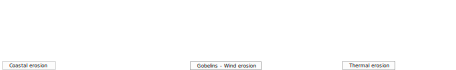
\includegraphics[width=\linewidth]{figures/teaser.pdf}
	\centering
	\caption{Applying shading and textures on the generated geometry can produce a plausible aspect of a coast eroded by waves on a long timespan, or a desertic landscape eroded by wind, or a mountainous area flatten by thermal erosion.}
	\label{fig:closerImage}
	\label{fig:teaser}
	
\end{figure*}

\section{Introduction}
Automated terrain generation is a key component of natural scene digital modeling for animated movies and video games. A standard approach is to first generate a base terrain geometry using noise to define the height on the input domain \cite{Musgrave1989, Olsen2004, Roudier1993}, the result will most likely lack realism and feel synthetic. Erosion simulation algorithms are applied, to simulate thousands of years of ageing by reproducing physical phenomena - i.e. effects of the elements (rain, wind, running water...) - affecting the terrain making it more believable \cite{Stachniak2005, Smelik2009, Galin2019}.\\
The process of terrain alteration caused by the effect of water, air, or any other element - natural or not - over time is usually performed in three steps \cite{Neidhold2005}: \textbf{detachment} - pieces of the ground of variable dimensions, ranging from complete ledges to grains of sand, are removed from the terrain depending on the simulated meteorological phenomenon - \textbf{transport} - pieces of ground fallen from their initial position are moved to a different one (e.g. a cornice falls down a slope or a grain of sand is thrown into the air) - and \textbf{deposition} - transported pieces of land are accumulated at a new part of the landscape. Various phenomena can cause these alterations: \textbf{thermal erosion} (bursting of rocks caused by expansion of water under frost, then falling of debris to the bottom of a slope), \textbf{hydraulic erosion} (detachment caused by the impact of water particles on surfaces and the transport of sediments by the flow of runoff), \textbf{wind erosion} (fine particles carried away in the wind and hit surfaces on their way, creating new fine particles which then also fly away), \textbf{chemical erosion} (chemical decomposition of rocks caused by rainwater or other fluids), other exceptional phenomena such as avalanches, animals, lightning, etc... modify the terrain \cite{Cordonnier2017a, Argudo2020, Cordonnier2018a, Cordonnier2017, Cordonnier2018}. 
\begin{figure*}
\centering
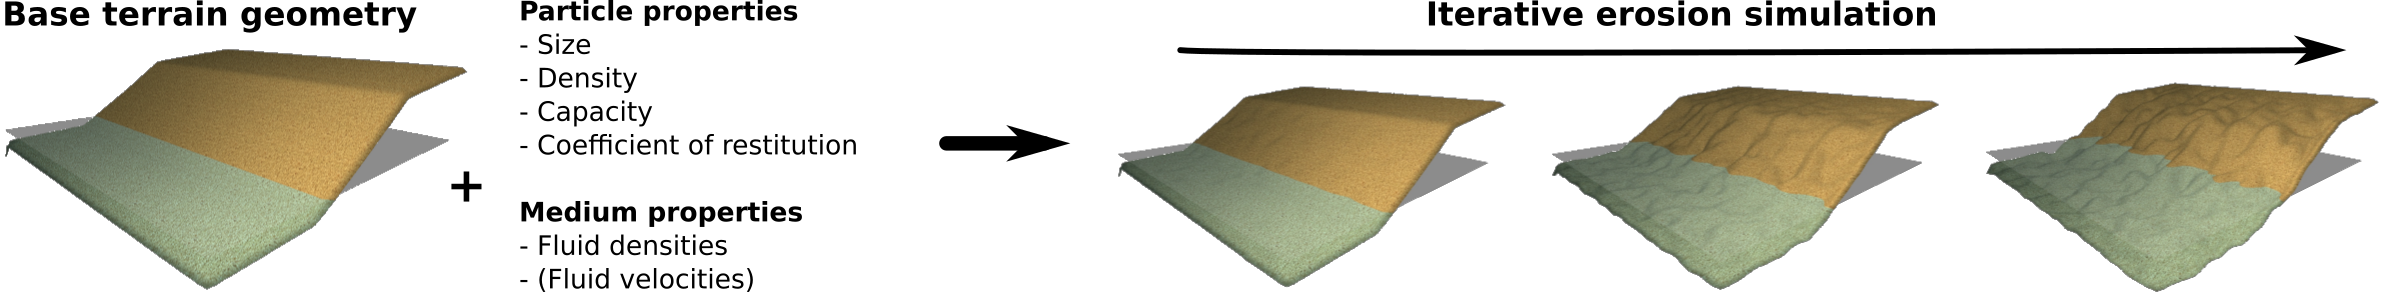
\includegraphics{figures/pipeline.png}
\caption{Our method require a base geometry, a small number of parameters for the particles and the medium used for the erosion simulation. It can be easily adapted to be compatible with different mediums and terrain representations.}
\label{fig:pipeline}
\vspace{-0.6cm}
\end{figure*}

In practice, the core idea to simulate erosion is to add or remove material from the terrain at given positions on the interface between the terrain and fluid eroding it (e.g. air or water). Hence, the two major problems to tackle are: how to locally alter the terrain geometry for material detachment and deposition and where to perform these alteration given the properties of the environment (terrain slope, fluid density and velocity).
A terrain is more than often represented in 2.5D using a 2D image called a heightmap which grey scale values define terrain elevation. While being the major terrain representation, only a limited number of environments can be modeled. Indeed, natural landscapes are intrinsically 3D (overhangs, cavities or geological structures such as arches or gobelins), this is particularly true for underwater environments generation. Alternate representation such as voxel grids, material layers or implicit surfaces can be used. A wide variety of method have been proposed to simulate natural erosion phenomena on heightmaps as the partial differential equations to model erosion can be discretized and solved in 2D and the material detachment and deposition at a given point of the terrain surface can be easily performed by elevating or lowering the ground level i.e. changing locally pixel intensities. 
For volumetric representations, the alteration of the terrain is not as trivial.
To define where to perform the erosion process the local slope variations are more than often used combined with eroding medium information. This fluid can be simulated using particle systems, Smoothed Particle Hydrodynamics (SPH) \cite{Kristof2009} or approximated using a simple vector field. 
Proposed methods offer a specific erosion effect tailored to a single terrain representation and fluid simulation.

In this work we propose an approach to simulate a large part of the geomorphological and meteorological phenomena present in the literature of terrain generation (including 3D and volumetric effects). We introduce a generalized algorithm performing the three stages of erosion on surface and volume representations alike, and expose very few intuitive parameters to be adjusted by the user (Figure~\ref{fig:pipeline}).
We propose to tackle separately the material variation and the fluid simulation. Our method relies on a particle system to simulate eroding agents, each thrown particle will collide with the terrain, perform terrain alteration at the collision point and transport material along its path. 
Their motion is computed using simple particle physics accounting for the medium density and particle properties (buoyancy and gravity forces). We consider each particle as independent, hence, they do not interact with each other, no collision detection or response. This simplification allows for efficient parallel computation. 
When more accuracy or control is needed, we propose to provide a vector field used to modify the particle speed at each time step. The nature of this vector field is flexible, it can be computed using a more or less accurate fluid simulation (SPH, FLIP,...) or be manually defined by the user. We propose a particle-based strategy for material alteration that can be applied on surface and volumetric representation. \\
The main contributions of this paper are: 
\begin{itemize}
\item a generalized particle-based algorithm performing the three
stages of erosion on surface and volume representations,
\item decoupling the erosion system from the fluid simulation, making the process more flexible in its usage and implementation and opening the door for richer effects that can easily be produced.
\end{itemize}
% -----------------------------------------------------------------
\section{State of the art}
\label{sec:state_of_the_art}
In this section, we first present the major terrain representations (height fields, layered representations, voxel grids, and scalar functions) and a subset of the major simulated phenomena used to erode terrains. We highlight the fact that, in the literature, a specific erosion method tailored to a given terrain representation is proposed for given phenomena which might lead to limitation in term of terrain modeling. Indeed, changing representation costs information and precision loss.
\subsection{Terrain Representations}
A terrain can be represented in various ways, each of them suited for a given application of which we give an brief overview, more details can be found in \cite{Galin2019}.\\
\textbf{Height Fields} represents the surface of the terrain by defining the elevation at each point in a 2D grid. This representation is simple, regular, and fast to process allowing for easy manipulation, such as raising or lowering the terrain \cite{Gain2009, Emilien2015}.\\
\textbf{Layered Representations} are an extension of height fields using a 2D grid where each cell represents a stack of different materials instead of a simple height \cite{Peytavie2009, Benes2001} allowing for memory efficient representation of volumetric terrains. To create complex structures, arches or caves, solid materials can be transformed into more granular ones, that can be stabilized \cite{Peytavie2009}.\\
\textbf{Voxel Grids} are regular, uniform volumetric grids that encode information on the presence or absence of material for each 3D point in the domain. Voxel grids are advantageous due to their regularity \cite{Dey2018} and ability to represent volumetric models at the cost of high memory footprint, which has limited their use in terrain generation \cite{Ito2003, Kaufman1993, Lengyel2010a}. We consider two voxel grid representations : \textit{density-voxel} grids for which each voxel contains a scalar value, for instance the occupation percentage \cite{Eisemann2008}  and \textit{binary voxel} grids that can be seen as a mask containing the presence of material information.\\
\textbf{Implicit terrains} represent landscapes as an implicit surface defined by a scalar function. This allows for high definition large terrain modeling. The application of combinable scalar function overlays \cite{Guerin2016a} or the definition of user-defined gradients \cite{Guerin2022} can be used to create complex terrain features. Altering a implicitly defined surface is a challenging task hence limited option exist for erosion simulation \cite{Paris2019}.

\subsection{Erosion Processes}
Erosion processes play a crucial role in shaping landscapes over time. We present different kind of erosion and how they apply to given terrain representations. Note that using existing methods all erosion methods can not be used on all representation.\\
\textbf{Thermal Erosion} is driven by large temperature shifts, transferring material based on slope thresholds. The process is iterative, redistributing material until slopes stabilize. It can be computed efficiently on height fields and layered terrains due to their manipulable height nature \cite{Musgrave1989, Benes2001, Peytavie2009}. However, its application on voxel grids is challenging due to limited Z-axis resolution.\\
\textbf{Hydraulic Erosion} stems from water movement, eroding and depositing sediment based on water flow intensity. 2.5D terrains are widely studied for this simulation, using either water slope velocities \cite{Neidhold2005} or water simulations for erosion effects \cite{Mei2007}. For smaller scales, 3D fluid simulations on voxel grids have been proposed \cite{Benes2006}. Kristof et al \cite{Kristof2009} used SPH (Smoothed Particle Hydrodynamics) for meshless erosion simulations on various terrains. Their method involves numerous particle interactions, demanding significant computational power. Our approach draws inspiration from this but enhances efficiency by removing certain particle interactions.\\
\textbf{Wind Erosion} shifts material through wind force, notably impacting areas with fine surface particles like deserts. It has been modeled on discrete height fields \cite{Roa2004, Paris2020} by mimicking sand's wind-driven trajectory and using thermal erosion for corrections. This process is simulated by iteratively displacing small amounts of matter, which make it less suitable for representations with discrete height resolution.\\
\textbf{Erosion by Other Forces} includes influences like glaciers, snow, tectonic movements, and fauna, each introducing distinctive terrain patterns, enriching its intricacy \cite{Cordonnier2017a, Cordonnier2023, Cordonnier2018a, Cordonnier2017, Cordonnier2018, Schott2023}. However, most methods are tailored by a given terrain representation, often the height fields, and might not be applicable to other representations due to their intrinsic properties.
%--------------------------------------------------------------------------
% \section{Technical background}
\section{Particle erosion}% [instead of "Technical background"]}
\label{sec:method}
Erosion occurs in three stages: material detachment, transport and deposition (respectively in red, black and green in Figure~\ref{fig:ablation_erosion}). In our approach, particles move through the medium following its flow (i.e. wind in air or currents in water) and then absorb or deposit a small amount of material upon contact with the land surface, effectively fulfilling the three stages of erosion.
\begin{figure}[h]
\vspace{-0.4cm}
\centering
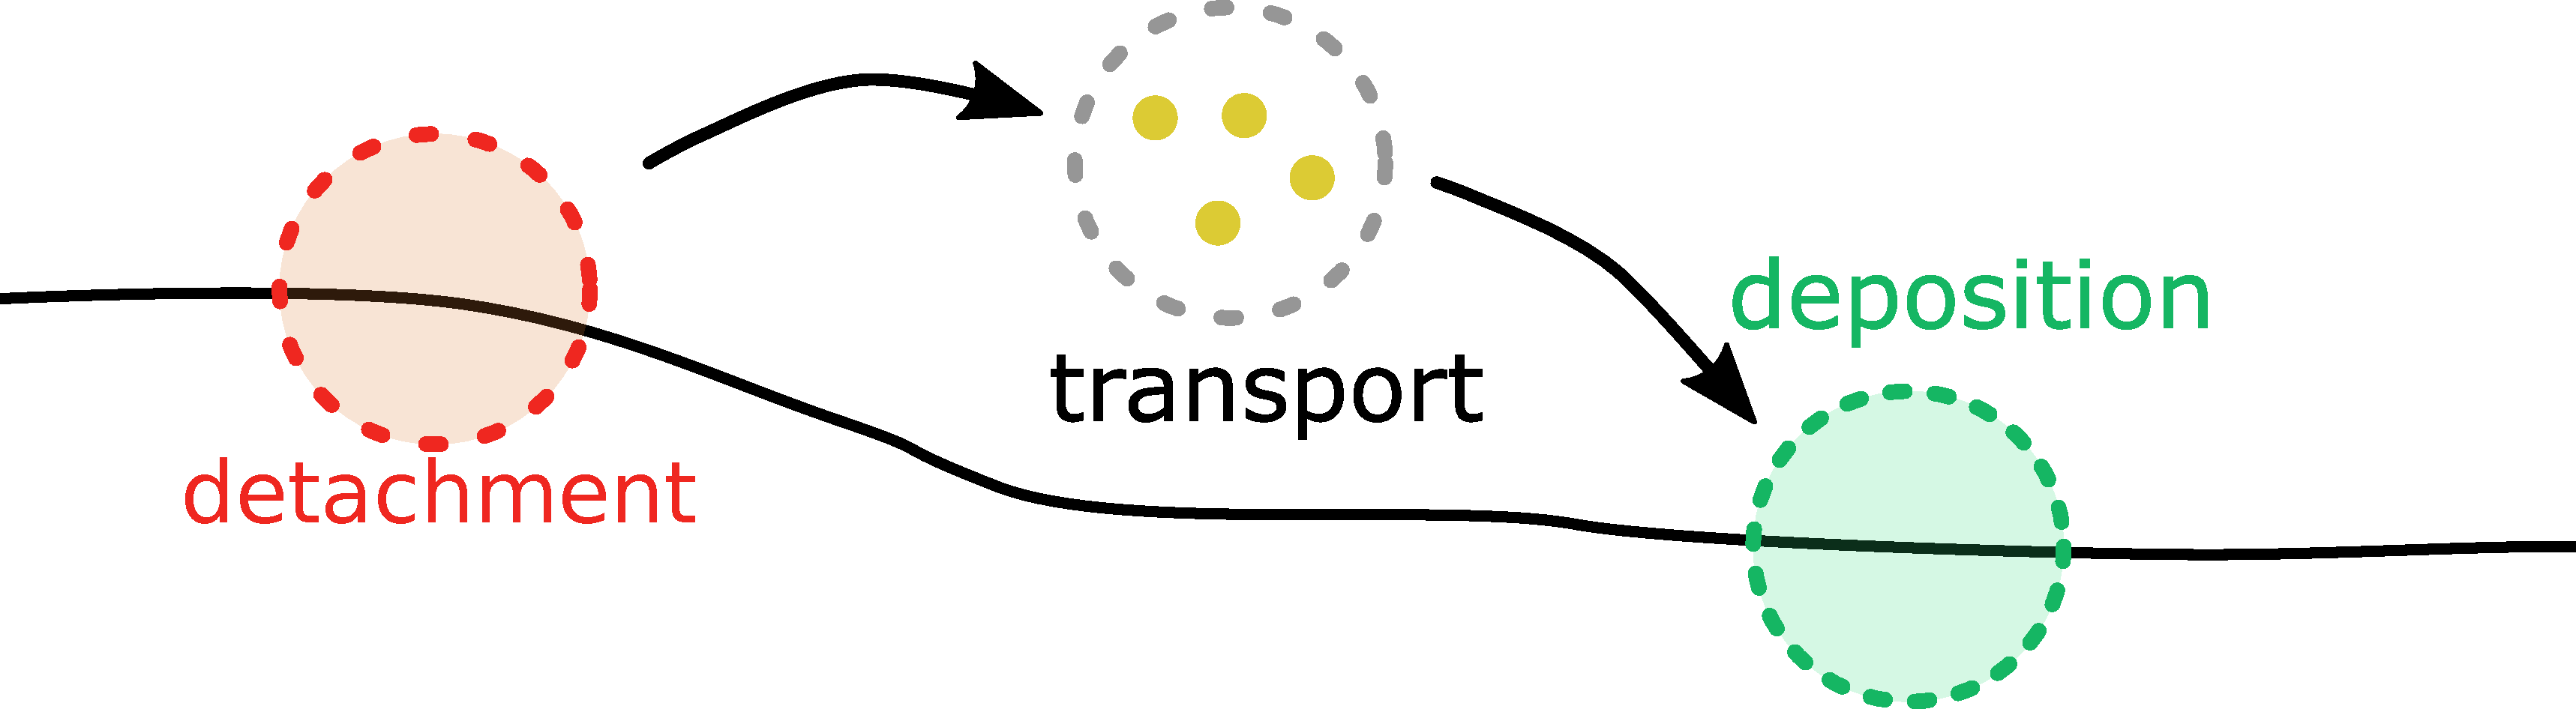
\includegraphics[width=0.95\linewidth]{figures/ablation_erosion.pdf}
\caption{Three steps of the erosion process from the sediment point of view: detachment from its original location - dotted red circle -, transport in a fluid - dotted black circle -, deposition at a new location - dotted green circle.}
\label{fig:ablation_erosion}
\vspace{-0.4cm}
\end{figure}
\subsection{Overview}
Particles are transported through the medium and can pass through several different media. Each medium is defined by a density and a flow. Consider, for example, water density to be \SI{1000}{\kilogram \per \cubic \meter} and that of air to be \SI{1}{\kilogram \per \cubic \meter}. The gravity applied to the particles is then very different between open and submerged environments due to the difference in buoyancy, while the process remains similar.
Using a pre-calculated flow field to guide particle movement simplifies the simulation by treating particles as independent entities, eliminating the need for inter-particle calculations. This not only reduces significantly the overall execution time but also offers users high flexibility over the quality of the simulation and simplify the implementation. 
\subsection{Erosion process}
\begin{wrapfigure}{r}{2,4cm}\vspace{-.5cm}
\centering
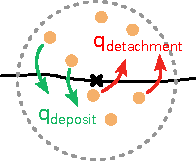
\includegraphics{figures/erosion_deposition.pdf}
\vspace{-.9cm}
\end{wrapfigure}
Every time the particle hits the ground, a given amount $\erosionAmount$ of sediment is detached from the ground (red arrows) while another amount $\depositAmount$ of sediments is deposed at this location (green arrows). Our erosion model is based on the work of Wojtan et al where \replace{a}{} regular 3D grids are used to estimate the fluid velocity and sediment transport \cite{Wojtan2007}. In the spirit of \cite{Kristof2009}, we transposed their method into a particle-based erosion simulation, but, in our proposition, we decouple the particle system from the fluid simulation, making the process more flexible and opening the door for richer effects that can easily be produced. 

\textbf{Detachment.}
As a particle approaches the surface of the terrain, its motion applies friction at the interface between fluid and ground, causing bedrock to dislocate microscopic parts, that we call abrasion. We use pseudoplastics model to approximate the amount of matter removed due to the shear forces while considering the physical properties of the fluid and the ground \cite{Wojtan2007}. 

The shear rate $\theta$ is approximated by the relative velocity of the fluid to the solid boundary $\velocity_{rel}$ over a short distance $l$.
We approximate the shear stress $\shearStress$ at the solid boundary by a power-law:
\begin{align}\label{eq:shearStress}
\shearStress = \shearStressConstant \theta^n
\end{align}
where $\theta = \velocity_{rel}/l$, $\shearStressConstant$ is the shear stress constant (often set to $1$) and $n\in[0,1]$ is the flow behaviour index. Shear-thinning models typically assume $n$ close to $\frac{1}{2}$, which is why we used this value as a constant.  

We can then compute the erosion rate $\erosionRate$ at any contact point between a fluid and a solid boundary using \eqref{eq:shearStress} by 
\begin{align}\label{eq:erosionRate}
\erosionRate = \erosionStrength (\shearStress - \criticalShearStress)^a
\end{align}
with $\erosionStrength\in[0,1]$ a user-defined erosion constant, $\criticalShearStress$ the critical shear stress value for which the matter starts to behave like a fluid and $a$ a power-law constant, typically considered as $a = 1$. 

In our method, the eroded quantity is approximated as the material contained in the half sphere, of radius $\particleSize$, in the normal opposite direction at the particle impact point (Figure~\ref{fig:erosion_heightfield}). We then use \eqref{eq:erosionRate}: 
\begin{align}\label{eq:erosionAmount} 
\erosionAmount = \erosionRate \frac{ 2 \pi \particleSize^3 }{ 3 }
\end{align}
to get the final eroded amount $\erosionAmount$. The particle is also defined by a maximal amount of sediments that can be contained in its volume before being saturated noted $\maxCapacity$. Note that this constant will be used for the settling velocity computation \eqref{eq:initialSettlingVelocity}.

\textbf{Deposition.}
The eroded sediments are considered in suspension in a fluid and are affected by its velocity. A fluid particle then transports the sediments in its flow until gravity settles it onto the ground again. The effect of gravity is modeled by a settling velocity $\settlingVelocity$ defined in Eq~\eqref{eq:initialSettlingVelocity}. We consider that the amount of sediment settled is proportional to the norm of the settling velocity as proposed in \cite{Wojtan2007} with $\depositionRate \in [0,1]$: 
\begin{align}\label{eq:deltaDepositon}
\depositAmount = \depositionRate ||\settlingVelocity||.
\end{align}
% The corrosion simulation can be performed by setting $\lambda_{deposit} = 0$.

\vspace{-0.4cm}
\subsection{Transport}
Our simulation is computed by integrating the full trajectory of multiple particles at each iteration unlike most other erosion methods. This allows to constantly have a terrain in a plausible state, while giving the possibility to increase the aging effect by running more iterations. 
Note that, reducing progressively the overall erosion strength can be used as a strategy to adapt the computation time to a chosen level-of-details.

We first present how to compute the particle speed using particle's physics then how to add optional medium velocity field to add a fluid simulation or user control.

\textbf{Particle's physics.}
From its independence with other particles: we consider each particle following Newton's laws of motion.\\
First, we define the external forces $\extForce$ applied on each particle, we consider gravity and buoyancy.
We calculate the buoyancy force $\buoyancy =-\fluidDensity V \vec g$ with $\fluidDensity$ the density of the fluid, $V$ the volume of the particle and $g$ the gravitational acceleration, but we can also calculate the force of gravity $\gravity = \particleMass \vec g$ with $\particleMass$ the mass of the particle. We then have the final external force $\extForce = \vec \gravity + \vec \buoyancy = \particleMass \vec g - \fluidVelocity V \vec g$ knowing the density of an object $\particleDensity = \frac{\particleMass}{V}$, we have:
\begin{align} \label{eq:gravity}
\extForce = V \vec g (\particleDensity - \fluidDensity ).
\end{align}
The particle velocity $\velocity$ can be integrated from \eqref{eq:gravity} by: 
\begin{align} \label{eq:velocity-computation}
\velocity = \int{ \extForce \, dt} + \settlingVelocity + \velocity_0,
\end{align}
with $\settlingVelocity$ the settling speed of sediments in a fluid with a viscosity $\mu$ given by Stoke's Law \cite{Stokes1850}: 
\begin{align} \label{eq:initialSettlingVelocity}
\settlingVelocity = \frac{ 2 }{ 9 }  g \particleSize^2 \frac{(\particleDensity - \fluidDensity)}{\mu } f(\capacity).
\end{align} 
We use the Richardson-Zaki relation as the hindered settling coefficient: \\$f(\capacity) = 1 - \left( \frac{\capacity}{ \maxCapacity } \right)^{n}$ \\with $\capacity$ and $\maxCapacity$ respectively the fraction of volume of sediments contained and the maximal fraction of sediments the particle can contain, and $n$ an exponent typically 4–5.5, which we set to 5 \cite{Richardson1954, Wojtan2007}.

Finally, the particle position can be integrated as: 
\begin{align} \nonumber
p = \int{ v \, dt} + p_0.
\end{align}
% $$p = \int{ v \, dt} + p_0.$$ \\ 
When the particle hits the ground, a coefficient of restitution affects its behaviour by reducing its velocity post-collision. This value depends on ground material as it is influenced mainly by the material's particle shape, coefficient of friction and density \cite{Yan2020}. Less bouncy particles lose speed quickly and settle down sooner, forming a steeper pile (Figure~\ref{fig:coefficient of restitution-diagram} blue), or a higher talus angle like chalk. On the other hand, more bouncy particles disperse more widely upon hitting a surface, resulting in a gentler accumulation like clay (Figure~\ref{fig:coefficient of restitution-diagram} red).
\begin{figure}
\centering
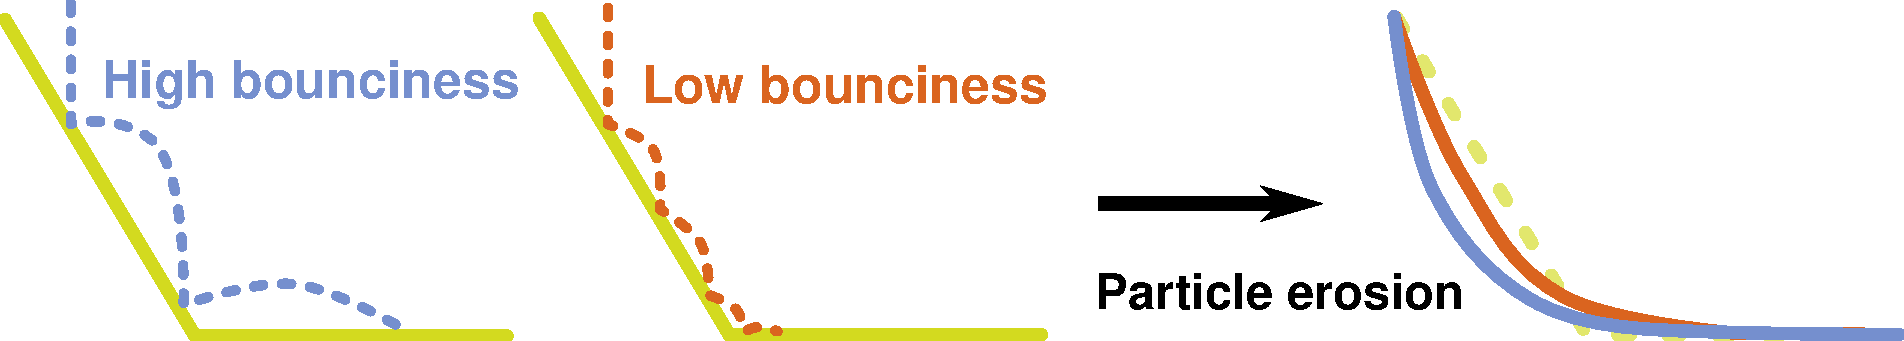
\includegraphics{figures/bounciness.pdf}
\caption{The coefficient of restitution affects the amount of energy absorbed from the particle when hitting the ground. Here, rain is applied on an initial slope (yellow). Only two particles are displayed, with a high (blue) and low (red) coefficient of restitution. The resulting slope after erosion is displayed in blue and red (right). }
\label{fig:coefficient of restitution-diagram}
\vspace{-0.4cm}
\end{figure}

\textbf{Velocity field.}
\label{sec:velocity_field_refinement}
In our model, we allow the user to add a velocity field to the environment that influences particles motion. This velocity field can be the result of a complex fluid simulation, a uniform vector field, or an artistic motion field.
We modify Equation \eqref{eq:velocity-computation} such that the particle's speed will be influenced by the velocity field as follows:
\begin{align} \label{eq:velocity-computation-final}
\velocity = \int{ \extForce \, dt} + \settlingVelocity + \alpha \fluidVelocity + \velocity_0,
\end{align}
with $\fluidVelocity$ medium velocity field modulated by $\alpha\in[0,1]$. 

Our particle system can model intricate scenarios, like the erosion caused by water currents on the seabed or aeolian erosion. The velocity field remains static during the erosion, which may cause inconsistencies in the fluid velocity field. However, minor changes can be overlooked to maintain a balance between realism and computational efficiency \cite{Tychonievich2010}. We offer several velocity improvement methods: \\
\textbf{-Fluid simulation refinement:} Many erosion systems incorporate fluid simulation, requiring regular updates for erosion and velocity \cite{Kristof2009, Wojtan2007}. Our method can use fluid simulations with multi-resolution refinement, with the possibility to focus the velocity field adjustments near the updated boundaries of the surface \cite{Roose2011}. \\
\textbf{-Particle velocities in fluid simulation:} With a Lagrangian fluid simulation relying on particle systems \cite{Koschier2022}, our particle velocities can be incorporated in its computation. This approach is only a provisional solution due to potential parameter mismatches with main fluid simulation. \\
\textbf{-Velocity field diffusion:} Given the minor changes to the surface level at each erosion iteration, which reflect the gradual alterations in terrain surface, we can estimate that the velocity at a fixed point transitioning between the inside and outside of the terrain closely mirrors the velocities observed in its surrounding area. In this context, we can simply interpolate the velocity field at any transitioning point. This simple method, as used in Figure~\ref{fig:underwater_result}, allows us to find a balance between achieving realistic flow simulations and maintaining computational efficiency.
% Our contribution part
% ------------------------------------------------------------
\section{Our erosion method}
\label{sec:application_on_representations}
\begin{figure}[t]
    \centering
    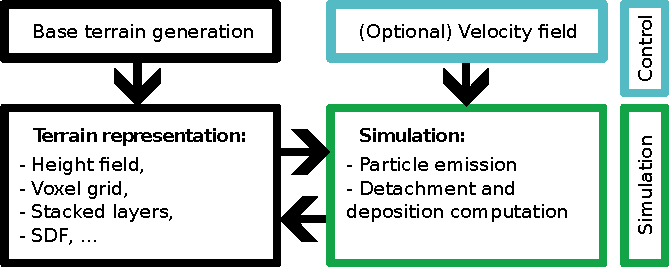
\includegraphics[width=\linewidth]{figures/figure_pipeline.pdf}
    \caption{Our overall pipeline: our erosion process compute matter displacement of a terrain using an arbitrary representation as long as intersections between particles and the ground can be detected. An optional velocity field, provided by the user, guides the particles trajectories. We propose surface alteration methods to apply the erosion to the terrain in a coherent way between possible representations. }
    \label{fig:figure_pipeline}
\end{figure}
In this section, we describe how to apply detachment and deposition to different terrain representations with our method (Figure~\ref{fig:figure_pipeline}). We cover the most commonly used representations namely height fields, layered terrains, voxel grid and implicit surfaces, note that our work could be extended to additional representations. Two conditions need to be satisfied for a representation to be eligible for our erosion method: being able to evaluate the intersection of a particle with the ground and compute the normal of the terrain at this point. To the best of our knowledge, all representation do. \\
We use Verlet integration for the particle's physics  \cite{Verlet1967}, with low error rate and stability even for high $dt$, reducing computation time for negligible imprecision \cite{Baraff1998, Swope1982}.

For all the representations, the amount of material absorbed by the particle, i.e. the erosion value $\erosionAmount$ from \eqref{eq:erosionAmount}, is taken around the particle at a radius $\particleSize$, meaning that the modification of the terrain by a particle at position $c$ will only occur for the positions $p$ satisfying $||p - c|| < \particleSize$. At the same time, the amount $\depositAmount$ from \eqref{eq:deltaDepositon} is deposited, resulting in a change $\totalErosion = \depositAmount - \erosionAmount.$\\ 
In our simulation, while the dynamics are informed by physical principles, the particle size is conceptualized within a dimensionless framework. This provides the flexibility to adapt our results to various real-world scales, ensuring the applicability of our model across diverse scenarios.
Note that, for a 2.5D terrain, we can consider that half of the sphere surrounding the particle is affected which has a volume of $V_{2.5D} = \frac{2 \pi \particleSize^3}{3}$ while a 3D terrain is affected by the full sphere $V_{3D} = \frac{4 \pi \particleSize^3}{3}$ (as illustrated  Figure~\ref{fig:erosion_heightfield}). In the following sections, we will describe the strategies used to modify the amount of matter for different representations. 
\begin{figure}
\centering
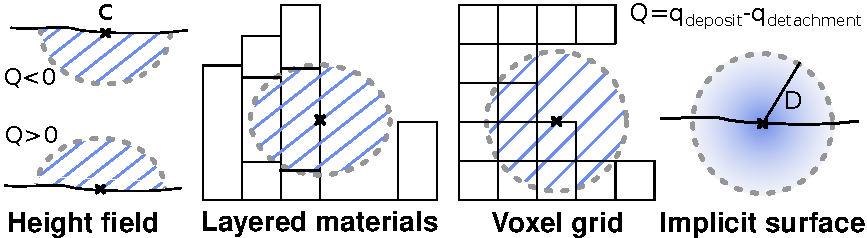
\includegraphics[width=\linewidth]{a_erosion_deposition.pdf}
\caption{Illustration of the material detachment in the (half-)sphere at contact point $C$ (cross) on different representations. (height field) When $Q<0$ material detachment happen in the bottom scaled half sphere of the particle's contact with the ground, while the deposition is applied on the upper half sphere of volume when $Q>0$. Unlike the height field, for 3D terrains detachment and deposit are applied in the full sphere around the contact point.}
\label{fig:erosion_heightfield}
\vspace{-0.5cm}
\end{figure}
\subsection{Application on height fields}
\label{sec:application_on_heightmaps}
On a height field defined by $h(p) = z$, the intersection point with the surface is verified at $p_z = h(p)$, and the normal can be computed at the intersection point. 

For this representation, the half sphere is scaled in the $z$ direction to fit $\alpha V = \totalErosion$ using $\alpha = \frac{\totalErosion}{V}$. We then can decrease the height $h'(p)$ at all points $p$ by the height of the scaled half sphere at position $p$. Given the height of the scaled half sphere of center $c$ and the distance of the particle to the center $d = ||p - c||$ by $h_{half sphere}(p) = \alpha \sqrt{\particleSize^2 - d^2}$ for all $p$ such that $d \leq \particleSize$ the radius around a particle.

This change of height can be sampled at all points of the 2D grid by reducing the height by 
\begin{align} 
\label{eq:erosionHeightfield}
\Delta h(p) &= \frac{\sqrt{\particleSize^2 - d^2}}{\alpha} = \frac{\totalErosion}{\frac{2}{3} \pi \particleSize^3} \sqrt{\particleSize^2 - d^2}
\end{align}
The height at each point after an erosion is then computed as $\Tilde{h}(p) = h(p) + \Delta h(p)$.

\subsection{Application on layered terrains}
\label{sec:application_on_layers}
Layered terrains are defined as $\mu: \mathbb{R}^3 \rightarrow \mathbb{N}$ assigning a discrete material index $\mu$ for any point in space \cite{Benes2001, Peytavie2009}. In the original work, outer borders stack elements of the terrain are transformed into density-voxels to enable global erosion through height changes. We enable the erosion/deposition process directly on the layers hence removing the need for representation changes. \\ 
When intersecting the terrain, the amount eroded for each material stack should be the integration of the volume of the intersection between the sphere surrounding the particle and the cubicle represented by the stack. Since there is no easy solution \cite{Jones2017}, we approximate the volume of the stack we need to alter using the previously defined height field equation \eqref{eq:erosionHeightfield}. 
At a distance $d$ from the particle, the height is defined as:
\begin{align} \label{eq:erosionLayers}
H(d) = \frac{|\totalErosion|}{\frac{2}{3} \pi \particleSize^3} \sqrt{\particleSize^2 - d^2}.
\end{align}
If $\totalErosion > 0$ (more deposition is applied that detachment) then we transform the materials in the stack contained in the sphere to become ground material. For $\totalErosion < 0$ the materials are transformed in background material.

\subsection{Application on implicit terrains}
\label{sec:application_on_implicit}
Implicit terrain are defined using a function $f(p)$ and its variation resulting from the erosion process using $\Delta f(p)$.
We propose a strategy to compute $\Delta f(p)$ at any point of the sphere surrounding the erosion point based on metaball primitives. At each contact point a metaball is added to create a hole or a bump in the terrain. A metaball is defined as: 
\begin{align}\label{eq:erosionMetaball}
\Delta f(p) = \frac{3 \totalErosion}{\pi} \frac{(1 - d)}{\particleSize}
\end{align}
with $d$ the distance of the point $p$ to the sphere center. For all point $p$ for which $d \geq \particleSize$, $\Delta f(p) = 0$ (see \ref{sec:appendix_metaball}).

As they are the most commonly used representations, we propose a formulation to erode implicit terrains defined by Signed Distance Functions (SDF) and by gradient or vector fields.

\textbf{Signed Distance Functions}
\label{sec:application_on_sdf}
Considering SDF, the terrain is defined as the 0-set of the signed distance function $f: \mathbb{R}^3 \rightarrow \mathbb{R}$, hence, for $f(p) = 0$, the inside as $f(p) < 0$ and outer-part (i.e. air or water) as $f(p) > 0$. \\ 
The particle erosion applies at impact points at discrete positions, so we propose to add or subtract metaballs defined using equation~\eqref{eq:erosionMetaball} to respectively deposit or erode material using a composition tree:\\ $metaball(p) = -\Delta f(p)$.\\
Now the eroded terrain function $\Tilde{f}(p)$ will be evaluated at each point $p$ from the initial terrain value $f(p)$, the erosion function $metaball(p)$ and the composition function $g(f_1, f_2)$:
\begin{align} \label{eq:finalMetaball}
\Tilde{f}(p) = g(f(p), metaball(p)).  \nonumber
\end{align}
As a metaball is added for each particle bounce on the terrain space partitioning optimization algorithms such as k-d trees, BSP trees or BVH can easily be used to improve performances.

\textbf{Other implicit terrains}
\label{sec:application_on_other_implicit}
are present in the literature, notably a 2.5D representation based on the surface gradient \cite{Guerin2022} and a 3D representation based on curves \cite{Becher2017} for which the trajectory of each particle projected to the closest surface could be used to define the alteration of the terrain.\\
In the case of gradient-based representation, we propose to use the partial derivative from the equation of the 2D scalar fields \eqref{eq:erosionHeightfield} that gives:
\begin{align} %\label{eq:erosion_gradients}
\nabla h' = - \frac{Q}{\frac{2}{3}\particleSize^3} \frac{1}{\sqrt{\particleSize^2 - d^2} } \vec{CP}
\end{align}
with $\vec{CP}$ the vector from the position $p$ to evaluate to the center of the erosion point $c$.
Now the new gradient field can be computed as: 
$$
\nabla \Tilde{h}(p) = \nabla h(p) + \nabla h'(p).
$$
\begin{figure*}
\centering
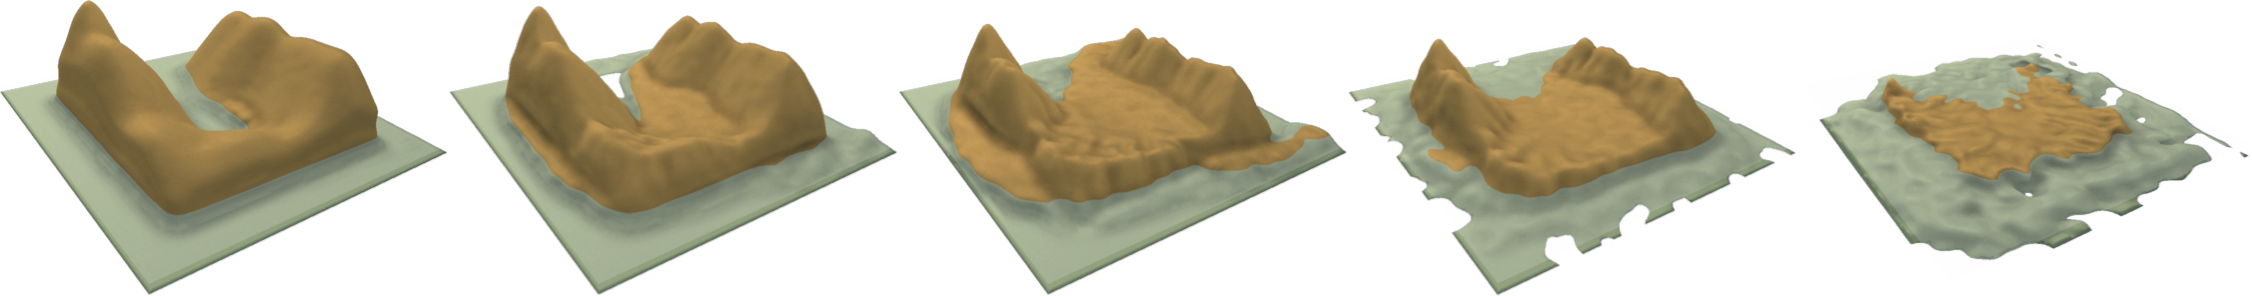
\includegraphics{figures/new_continuous_erosion2.png}
\caption{Our erosion method is applied iteratively on a completely synthetic island, the terrain is altered to obtain a plausible shape by forming rills. The use of particles with hydraulic densities dropped from the sky results in a strong erosion on the sides of the mountains, and the particles that slide to the sea are mainly drifting offshore resulting in the formation of small beaches and a weaker erosion on the bottom of the water body. Repeating the process causes the island height to decrease progressively up to the point where only the submerged part of the terrain is sheltered from erosion.}
\label{fig:continuous-erosion}
\vspace{-0.4cm}
\end{figure*}
\vspace{-0.6cm}
\subsection{Application on voxel grids}
\label{sec:application_on_voxels}
% \subsubsection{Density-voxels}
We consider two of the voxel grids representations: density-voxel grids and binary voxel grids for which we present our material alternation strategy.

\textbf{Density voxels.}
\label{sec:application_on_density_voxels}
We consider "density-voxel" grids defined on $f: \mathbb{Z}^3 \rightarrow [-1, 1]$ for which a voxel is be full for $f(p) = 1$, partially full for $-1 < f(p) < 1$ or empty for $f(p) \leq -1$. 
This definition allows us to erode them smoothly. 
Since this kind of grid is a discretizaion of a scalar function, We could directly use \eqref{eq:erosionMetaball}, as described previously, but we take advantage of the discrete nature of the representation to avoid expensive computation. \\
We apply the erosion from a particle at position $c$ on all points $p$ in the volume proportionally to the distance from the center of the sphere $d = ||p - c||$ to find an approximation to the real erosion value per voxel $q_{approx} = \totalErosion \frac{1 - d}{\particleSize}$.
Using their discrete nature, we rectify this value to sum up the total erosion value to $\totalErosion$ by dividing each value by the sum of the distances. We now consider eroding the "empty" voxels since their density can drop until $-1$. We then have for all surrounding voxels: 
\begin{align} \label{eq:erosionVoxels}
\Delta f(p) = \totalErosion \frac{ (1 - \frac{d}{\particleSize} )}{ \sum {(1 - \frac{d}{\particleSize})}}.
\end{align}
Resulting voxel value is computed as $\Tilde{f}(p) = f(p) + \Delta f(p)$.
In our implementation, when $f(p) > 1$, we simply transport the density excess to the above voxel, giving it a very close analogy to height fields as long as $|\Delta f| < 1$. 

\textbf{Binary voxels}
\label{sec:application_on_binary_voxels}
The terrain can be represented using an occupancy function as $f: \mathbb{Z}^3 \rightarrow \{0, 1\}$ where a voxel $f = 1$ defines the ground and $f = 0$ the background. \\ 
We propose to apply particle erosion by assigning voxels a number of hits, and transform them as air or as ground when this number reaches a critical value $C$ that is proportional to the particle's strength parameter $\erosionStrength$ \cite{Jones2010}. \\ 
On a hit, all voxels in a radius $\particleSize$ receive a hit number: 
\begin{align} \label{eq:erosionDiscreteVoxels}
\Delta hits = \lfloor \alpha \Delta f \rfloor
\end{align}
with $\Delta f$ the erosion per voxel computed using \eqref{eq:erosionVoxels} and $\alpha$ a coefficient high enough to obtain values above 1. \\ 
All voxels with $\# hits > C$ are transformed to background and voxels with $\# hits < -C$ are transformed to ground.\\
Note that, a binary voxel grid can also be transformed into a density-voxel grid to be eroded smoothly.

Our formulation for height fields \eqref{eq:erosionHeightfield}, can be used to erode 2D scalar field-based representations. Similarly, 
our proposition for SDF \eqref{eq:erosionMetaball} enables erosion for continuous 3D scalar fields and voxels \eqref{eq:erosionVoxels} for discrete 3D scalar fields respectively.
% -----------------------------------------------------------
\section{Results}
\label{sec:erosion_examples}
\begin{wrapfigure}{r}{3,5cm}
\centering
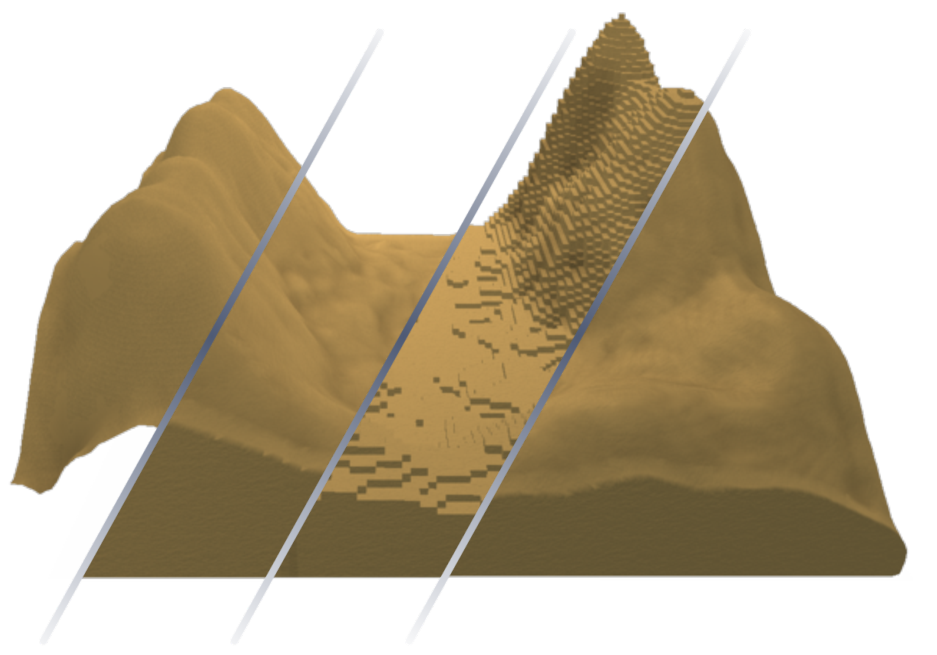
\includegraphics{figures/multi_representations.pdf}
\label{fig:comparison-representations}
\vspace{-1.0cm}
\end{wrapfigure}
Our erosion process enables the simulation of a wide range of erosion effects on the major terrain representations alike. In this section, we present applications that demonstrate the versatility of our method by changing the particle's effect size, quantity, density, maximum capacity, deposition factor and the velocity fields. The results of each process are presented in Figure~\ref{tab:result_figures}, parameters used are available at Table~\ref{tab:result_parameters}. 
It is important to note that all erosion examples presented in this section are available for any 3D terrain representation. However, we cannot create volumetric structure, such as overhangs, using 2.5D representations (height fields).

Environment density $\fluidDensity$ is set to \SI{1}{\kilogram\per\cubic\meter} above water level (terrain blue part) and to \SI{1000}{\kilogram\per\cubic\meter} below it.
Velocity field's refinement is done by using the presented diffusion strategy.

\begin{table*}
    \centering
        \begin{tabular}{|lHlllllllllllll|}
            \hline
            \thead{Name} & \thead{Results} & \thead{Rep.} & \thead{Dimensions} & \thead{Res} & \thead{$\#P$} & \thead{$\#N$} & \thead{$\particleSize$} & \thead{$COR$} & \thead{$\particleDensity$} & \thead{$\capacityFactor$} & \thead{$\erosionRate$} & \thead{$\depositionRate$} & \thead{Vel field} & \thead{$t$} \\
            \hline
            \exampleHydraulic \\
            \exampleCoastal \\
            \exampleMeanders \\
            \exampleRiverTwo \\
            \exampleLandslide \\
            \exampleVolcano \\
            \exampleKarstBinary \\
            \examplePipes \\
            \exampleWindErosion \\
            \exampleWaterCurrents \\
            \hline
        \end{tabular}
        \caption{Parameters used for the generation of the terrains presented in Figure~\ref{tab:result_figures}, with "Rep" the representation  (\heightmap: Heightmap, \densityVox: Density-voxels, \binaryVox: Binary voxels, \implicit: Implicit) "Res" the resolution in meter per voxel or cell, $\#P$ the number of particles per iteration, $\#N$ the number of iterations, $\particleSize$ the particles radius (in voxel or cell unit), $COR$ the coefficient of restitution, $\particleDensity$ the particle density in \SI{}{\kilogram\per\cubic\meter}, $\capacityFactor$, $\erosionRate$ and $\depositionRate$ respectively the capacity, erosion and deposition factors, "Vel field" the type of velocity field used and $t$ the computation time of the simulation in seconds on CPU. \\ $^{(1)}$ The velocity field is a vector field defined as $\fluidVelocity(p) = [0 ~ sin(p.x) ~ 0]^T$.}
        \label{tab:result_parameters}
        
\end{table*}

\textbf{Rain.}
Hydraulic erosion from rain is the most common process used in terrain generation. In this case, particles are seen as water droplets falling from the sky and rolling downhill due to the gravitational force of Earth. No velocity field is required from fluid simulation. These parameters result in a detailed geometry of the rills on the side of mountains that quickly emerge and deposit many sediments in the valley.  
We demonstrate the result of rain erosion in \referenceExemple{Rain} with a computation time of 4 seconds.  \\
Using this erosion parameters in combination with water bodies results in different outcomes (Figure \ref{fig:continuous-erosion}). The terrain above water is directly affected by the erosion process while particles colliding with the underwater part of the terrain are slowed down and filled with sediments, leading to mainly apply deposition. The result is a typical hydraulic erosion on mountains and the formation of slopes and beaches near water level.

\textbf{Coastal erosion.}
Waves repeated motion  creates coastal erosion, that can be seen as cliffs with holes at the water level. \\
We apply a uniform velocity field in the water pointing towards the coast to simulate waves and emit particles from the water area with a large size, a density between air and water densities, a high capacity factor and a low deposition factor $\depositionRate$. Using these parameters, the erosion process is focused at the interface of air and water, and apply a coarse detachment while depositing a very small quantity of sediments, simulating the corrosive effect of water on limestone. \\ 
This effect can only be simulated on 3D terrain representations, but will create cliffs on a 2D representation. 
\referenceExemple{Coastal} presents the result of coastal erosion on a density-voxel grid that creates overhangs around sea level using a small amount of particles. Note that, the same effect using an alternate implicit representation based on SDF is displayed in Figure \ref{fig:screen-paris2019-1}.
A shaded version of this effect is presented in Figure \ref{fig:closerImage}.

\textbf{Rivers.}
Given a source point, we generate particles that run downhill, simulating the formation of a river. More complex erosion simulation using fluid simulations like SPH \cite{Kristof2009} would create realistic results at the cost of high processing time. Our method offers the flexibility to be applied either with a velocity field (simple, used given or resulting from a fluid simulation) or without allowing for simplicity and efficiency.\\
When provided with a hand-made or procedural velocity field, our particle system can reproduce simple river meanders (\referenceExemple{Meanders}). \\ 
\referenceExemple{River} presents a river that has been modeled by emitting water particles with different sizes that ranges from \SI{1.5}{\meter} to \SI{5}{\meter}, a high coefficient of restitution and a low capacity factor. Random sizes are used to simulate a river for which the flow rate had fluctuated over formation time, while the low capacity ensure that the banks of the river stays smooth. A high coefficient of restitution is a strategy that let the particles flow with low friction, approaching a water behaviour. Our particles are affected only by gravity, without fluid simulation.

\textbf{Landslide}
are mainly caused by large amount of water saturating the ground and flowing downhill, transporting matter in its path. \\
By using water particles with a medium size, a low coefficient of restitution and a low capacity factor but a high deposition factor $\depositionRate$, they transport sediments on short distances as the velocity quickly drops to 0, and ground material is completely spread along its path since it is easier to deposit the same amount of sediment than the eroded amount at each collision point. Reducing the density of the particle simulates a rise of viscosity in the settling velocity formula, increasing again the quantity of matter to deposit at contact with the ground. By this means, we can simulate landslides as illustrated on \referenceExemple{Landslide}. A smoother surface is resulting, compared to the rain erosion as the rills are filled with sediments as soon as they begin to form.
%
By setting the initial capacity of the particle equal to 10\% of its max capacity, the mass of the terrain increases, simulating a volcano eruption as illustrated on \referenceExemple{Volcano}.

\textbf{Karsts} networks are created over hundreds of years from the corrosion of water on the limestone in the ground. A limited number of methods have been proposed for the procedural generation of karsts \cite{Paris2021}.\\ 
By reducing the deposition factor $\depositionRate$, the particles simulate corrosion (without mass conservation). We can use the same particle parameters than the coastal erosion (big size, a density between air and water densities, a high capacity factor and a low $\depositionRate$) and optionally provide a 3D shear stress map. The karst will automatically follow the softest materials, which is geologically coherent as given in example in \referenceExemple{Karst}, where we can observe a "pillar" that is formed in the center, and thus the karst forms two corridors that finally merge partially. 
%
Underground results are only available for representations allowing 3D structures. Another underground terrain simulation is shown in \referenceExemple{Tunnel} in which a water runoff is eroding a tunnel without the use of a fluid simulation. Here, when particles bounce often on the terrain surface, the coefficient of restitution may be seen as a viscosity parameter.

\textbf{Wind}
erosion is a significant process in desertscapes shaping since there are no obstacles on the airflow path. Air particles can reach high velocities, transporting sand over long distances forming either dunes or are blasted into rocks, eroding into goblins. \\ 
By setting the density of our particles close to \SI{1}{\kilogram\per\cubic\meter}, two erosion simulations can be applied at once. Air particles follow closely the flowfield given by the user in air. This flowfield can be given from a complex simulation, a user-defined wind rose \cite{Paris2020} or a random flowfield with a general direction. \\ 
The generation of the different sand structures depends on the velocity field provided, and a simple field will easily generate linear dunes. On contact with a rock block, the simulation will automatically erode block borders, creating shapes looking like gobelins. \\
\referenceExemple{Wind} gives an example of wind erosion on a flat surface with rock columns being eroded. Given a strong 2D velocity field computed by the high wind simulation proposed in \cite{Paris2020} is used on light particles, the simulation is fast thanks to the low number of collisions each particle has with the ground. 

\begin{figure}[b]
    \centering
    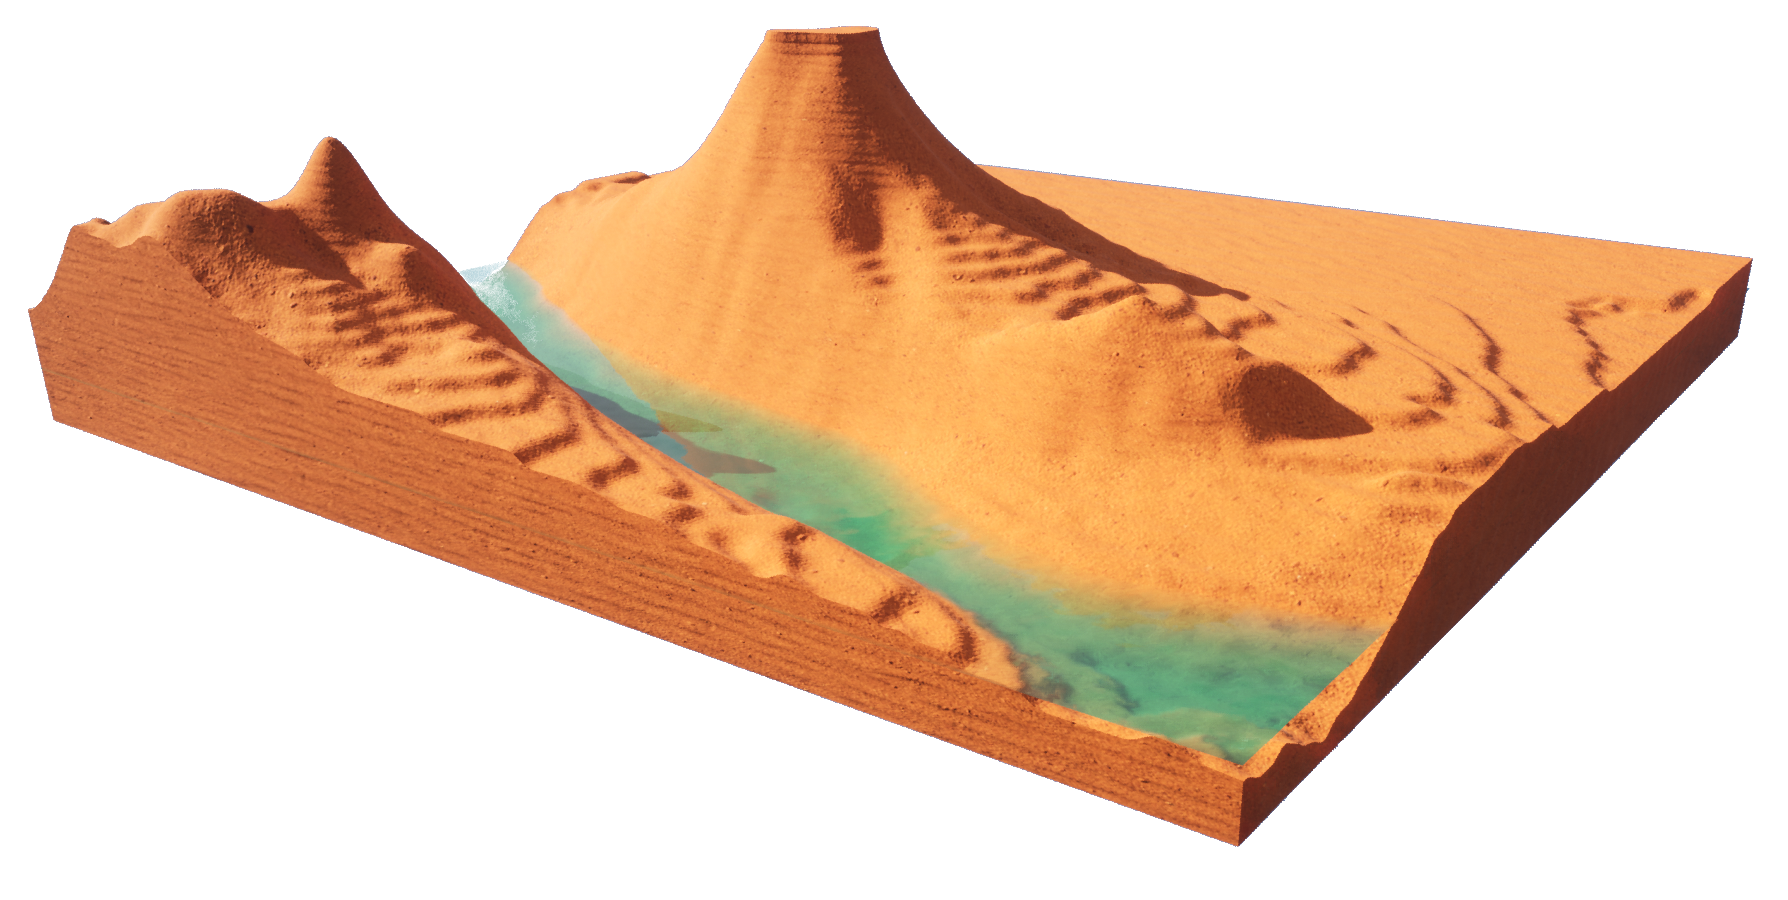
\includegraphics[width=0.49\linewidth]{Results/MultiEffects_base.png}
    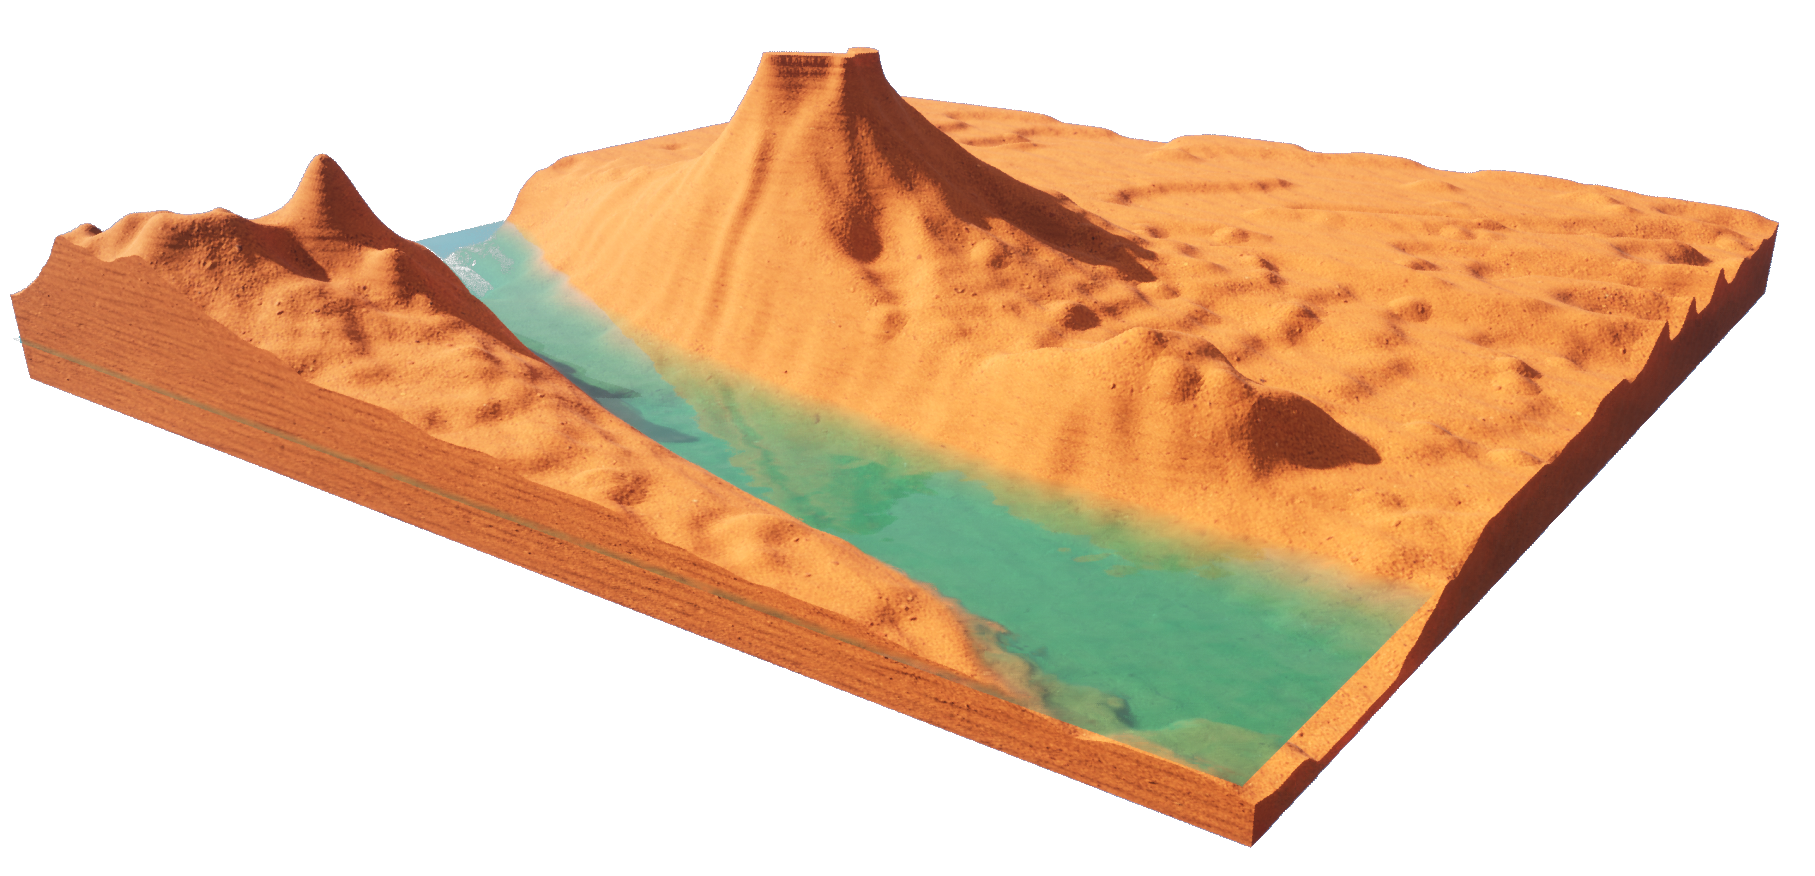
\includegraphics[width=0.49\linewidth]{Results/MultiEffects.png}
    \caption{Multiple erosion types can be combined. On an initial synthetic 500x500x50 density voxel grid, the a wind erosion is applied on the surface of the terrain while hydraulic erosion shapes the rills and the base of the mountains. A water current digs its borders and spreads sediments at the bottom. }
    \label{fig:multiErosions}
\end{figure}
\textbf{Multiple phenomena} A terrain eroded with multiple erosion phenomena applied on a 500x500x50 density-voxel grid is illustrated in Figure~\ref{fig:multiErosions}. Here, water-density particles are applying rain on the terrain while the coasts of the river are being eroded thanks to a velocity field defined at the water level. The velocity field defined in the air mainly affects particles with air-density, such that wind erosion can be applied at the same time. The computation of these effects took 7 seconds on CPU.

\textbf{Underwater currents}
Procedural generation of underwater 3D terrains has received little attention. The difference between the underwater and the surface rely on the buoyancy force that is much stronger, meaning that the water flow has a much more impacting effect on erosion than wind. Taking into account the density of the environment and the velocity field of water in our formulas are the keys to be able to apply any erosion in this environment. 
Our method works in a water environment by giving at least water density to particles. Given a velocity field describing underwater currents from a complex simulation or from a sketch, the particle system erodes the terrain. \\ 
In the example presented in \referenceExemple{Underwater}, the velocity field is given by a simple 3D fluid simulation \cite{Stam1999} applied on the terrain.

A complex water flow simulation is computed using SIMPLE \cite{Caretto1973} fluid simulation with OpenFOAM. The resulting erosion can then follow complex water movement and erode the terrain at the most affected parts of the 3D terrain as the trajectories of the particles (green) is highly affected by the fluid velocity (blue). The density of the particles and the environment being close, the buoyancy cancels most of the gravity force, leaving the velocity of the particles computed by the fluid velocity $\fluidVelocity$ and settling velocity $\settlingVelocity$ from \eqref{eq:velocity-computation-final} (Figure~\ref{fig:underwater_result}).
\begin{figure}[t]
    \vspace{-0.2cm}
    \centering
    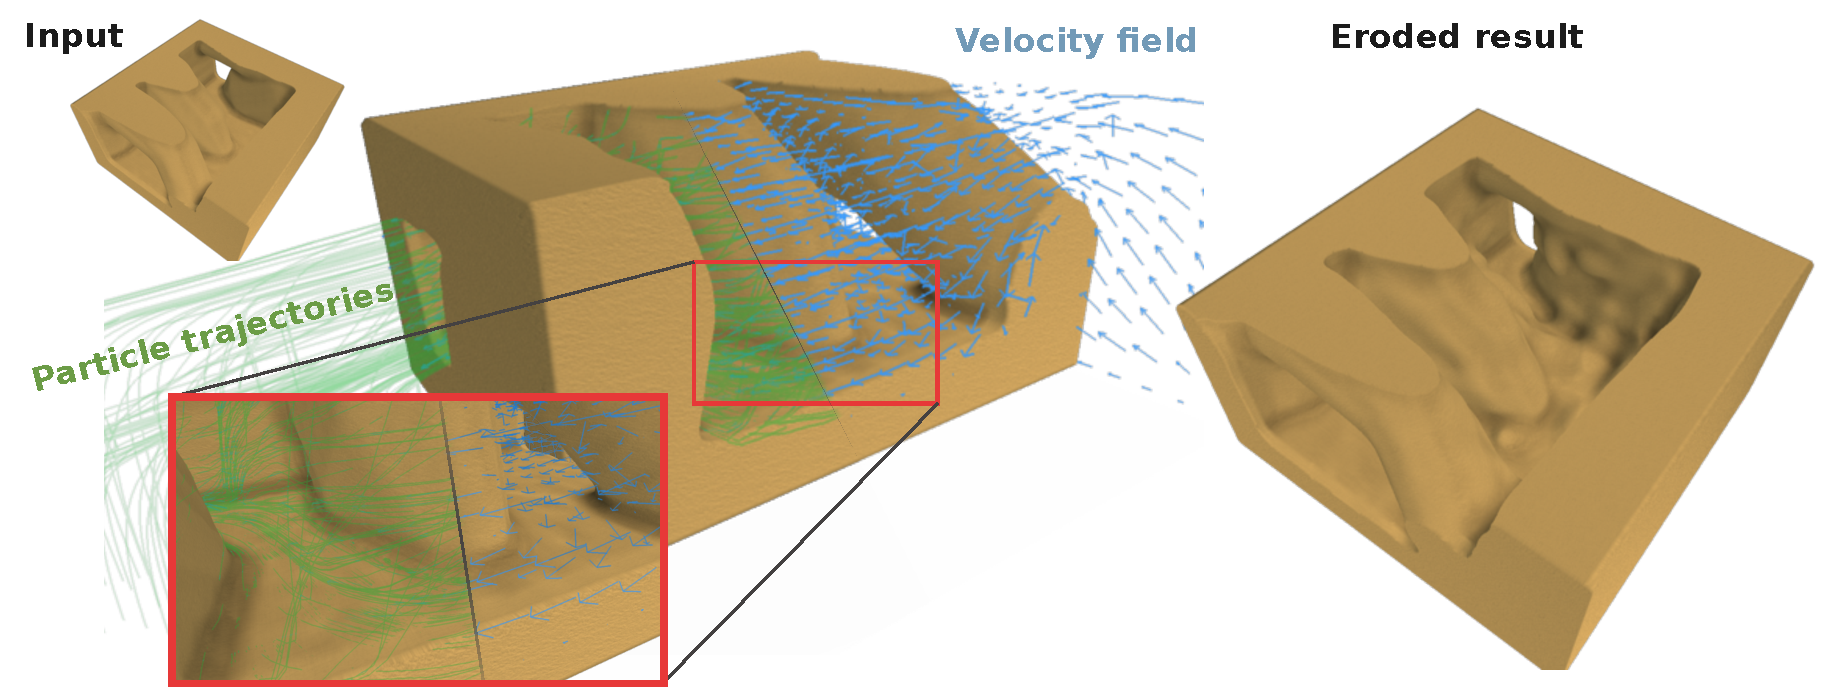
\includegraphics[width=\linewidth]{Results/flowfield.pdf}
    \caption{A complex water flow simulation is computed using OpenFOAM. Particle trajectories (green) are highly affected by the fluid velocity (blue). Most the terrain exposed surfaces is eroded (bottom). }
    \label{fig:underwater_result}
\end{figure}
% -----------------------------------------------------------------
\section{Comparisons}
In the following section, we compare our method with existing ones to show that while we are versatile on the terrain representation, we are also able to reproduce various effects without applying specific algorithms. The other works are displayed in blue to distinguish them from ours.

\textbf{Coastal erosion on implicit terrain representation:}
Paris et al present an erosion simulation method applied to implicit terrains able to create coastal erosion, karsts and caves by adding negative sphere primitive in the terrain's construction tree \cite{Paris2019}. The positions of the spheres are determined using a Poisson disk sampling at the weakest terrain area defined by the Geology tree of their model. They are simulating the corrosion effect of water on the rocks. Our work is also able to approximate this phenomena by defining the position of these sphere primitives at the position where the water particles hit the surface. While the computation time of the positions of the sphere is higher due to the fact that we are evaluating the position of our particles at every time step in the implicit model (which could be improved by the triangulation of the implicit surface, or better, a dynamic triangulation), the distribution of our erosion primitives is based on a physical model instead of a mathematical model, meaning that we can integrate more easily the direction and strength of the waves for example. The management of their sphere primitives can be replicated with our method by considering that a particle exists until a collision occurs, at which point it disappears. Their method is not conserving the mass of the terrain, which is acceptable for the corrosion simulation, but limits its validity for other erosion simulations. In our method, the particle can be tracked until it settles, ensuring mass conservation (Figure~\ref{fig:screen-paris2019-1});

\begin{figure}
\centering
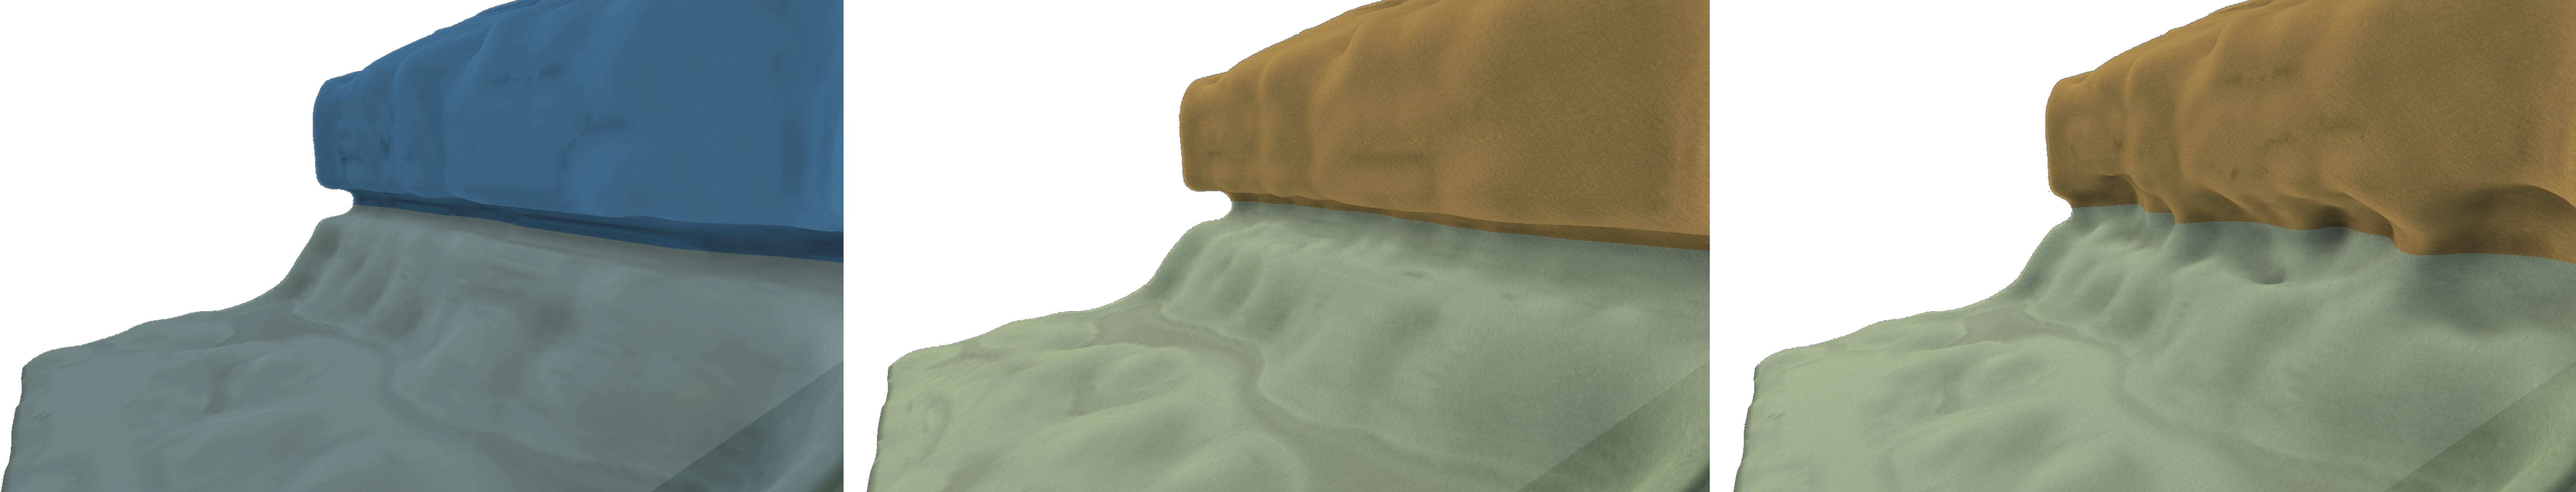
\includegraphics[width=\linewidth]{otherPapersRepro/costal.pdf}
\caption{The algorithm proposed by Paris et al \cite{Paris2019} allows for the simulation of coastal erosion (left) that we can reproduce almost identically by allowing our particles to collide only once with the ground and applying only erosion (center). If we apply our erosion with the full tracking of our particles and using deposition, we can achieve more diverse results (right).}
\label{fig:screen-paris2019-1}
\vspace{-0.5cm}
\end{figure}
%
\begin{figure}[t]
\vspace{-0.3cm}
\centering
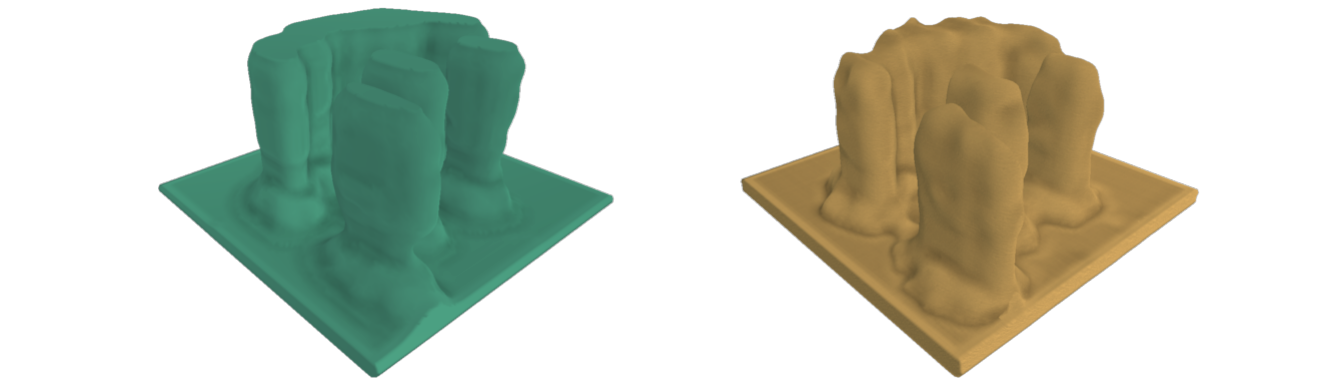
\includegraphics[width = \linewidth]{otherPapersRepro/gobelins2.png}
\caption{The algorithm proposed by Jones et al \cite{Jones2010} allows for an efficient simulation of the spheroidal erosion, making the creation of gobelins on voxel grids in a plausible way (left). Our algorithm naturally erodes the most exposed areas of the terrain when particles are affected by the wind (right).}
\label{fig:screen-jones2010}
\end{figure}
%
\textbf{Wind erosion on voxel grid representation: }
Jones et al propose a weathering erosion on voxel grids by approximating and eroding continuously the most exposed voxels \cite{Jones2010}. When a solid voxel is decimated, it is considered deposit and is displaced down the slope until a minimal talus angle in the terrain is reached and if the deposition is eroded again, it disappears. Our work is able to reproduce their algorithm by sending our particles from a close distance to the terrain surface. By doing so, we reproduce the erosion process as much as the deposition process since the air particles, filled with sediments, is falling automatically towards the local minimum of the erosion point. Just like in their work, we can easily define the resistance value of the materials to add diversity in the results. By adding the possibility of a wind field, even a very simple uniform vector field, to the simulation, we naturally add the wind shadowing effect that protects a gobelin surrounded by bigger gobelins, and also allows the deposit slope to fit more closely to the wind direction (Figure~\ref{fig:screen-jones2010}).

\begin{figure}[b]
\centering
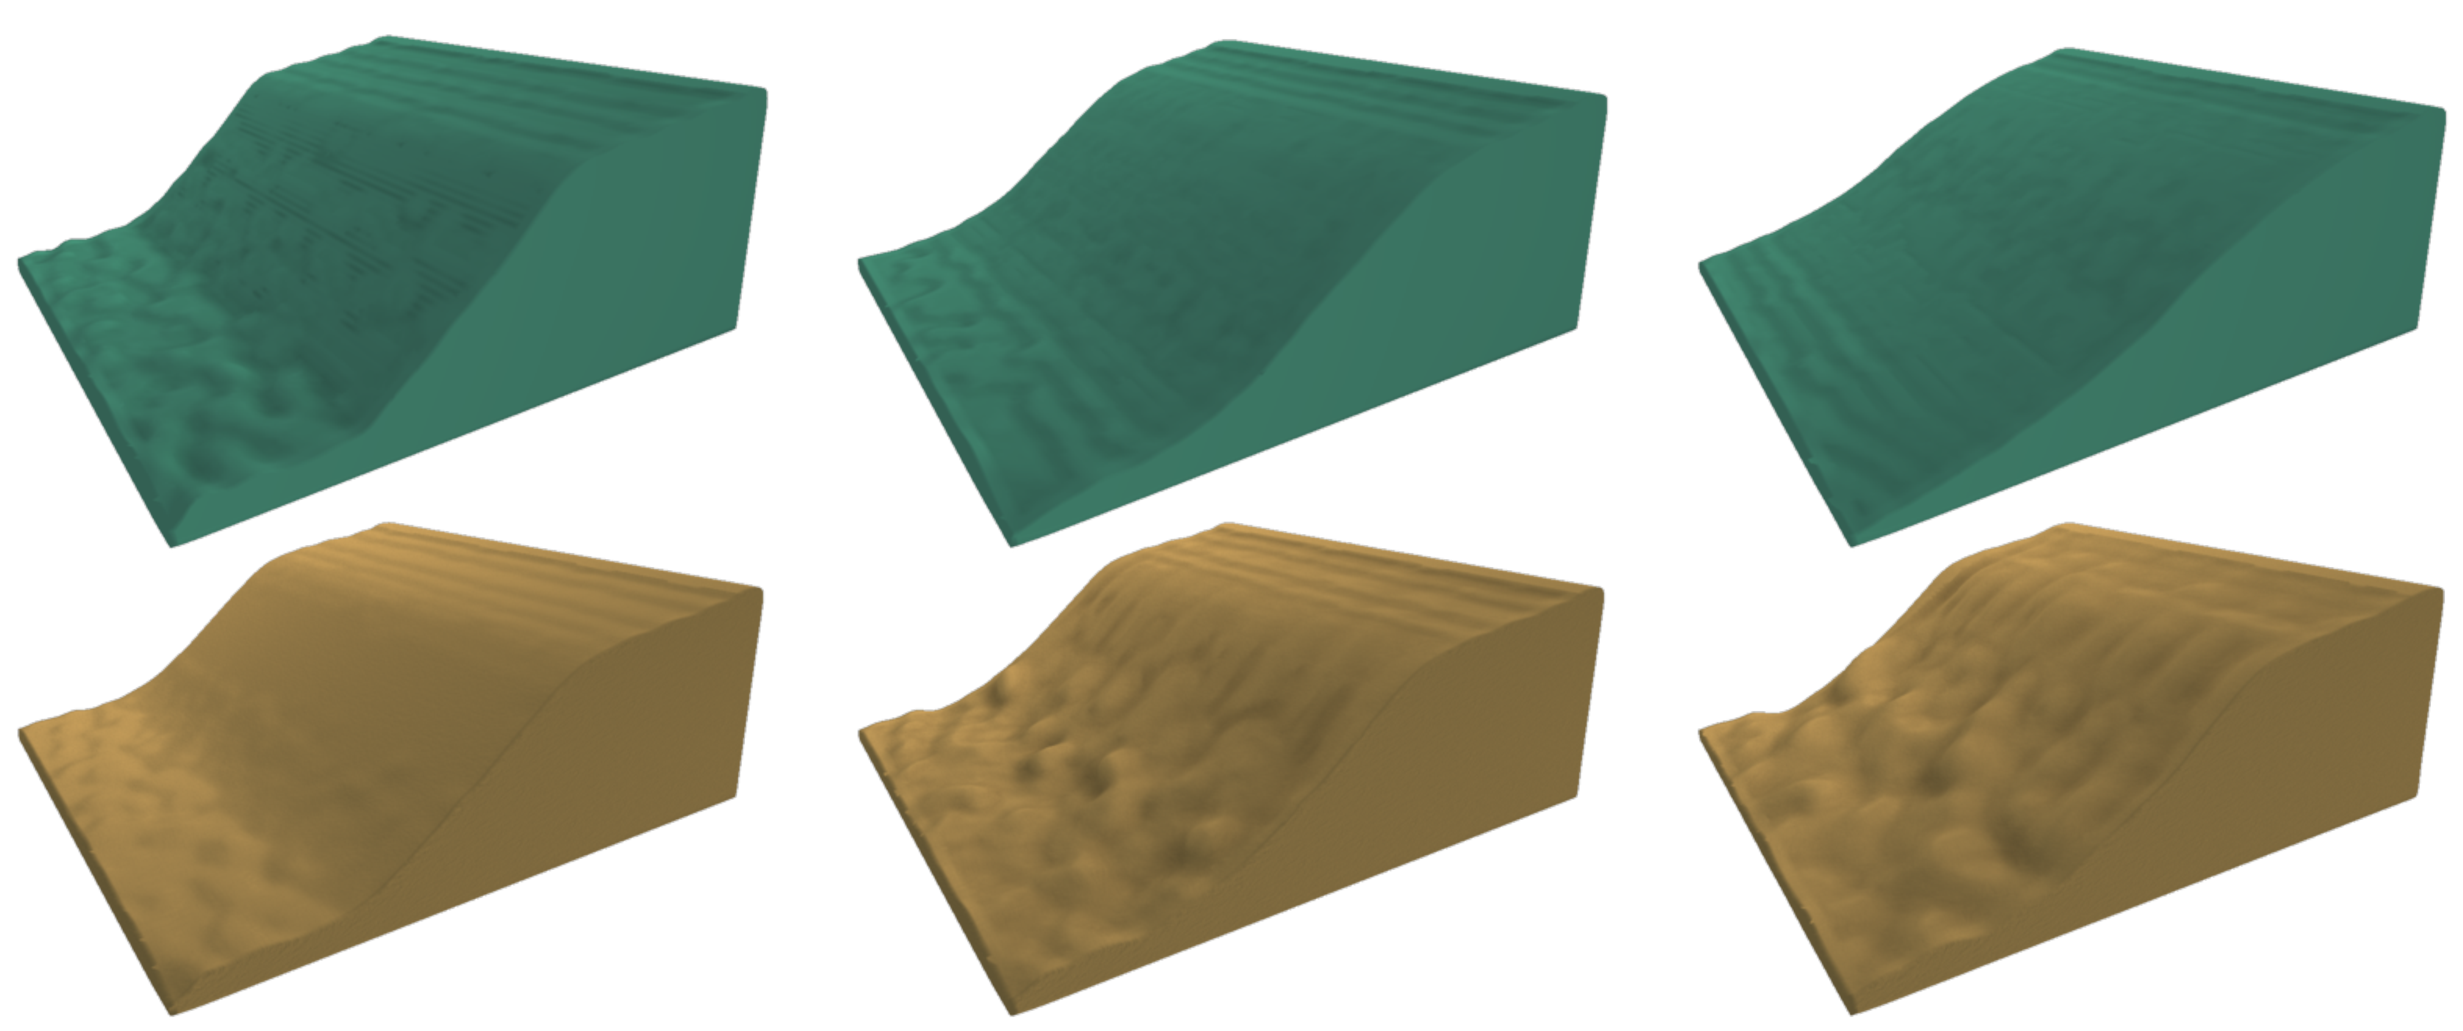
\includegraphics[width= 1\linewidth]{otherPapersRepro/hydro.pdf}
\caption{While our resulting geometry on the hydraulic erosion (bottom) is less smoothed than the one proposed proposed by Mei et al. \cite{Mei2007} (top), our method allows the application on more terrain representations than the height fields only.}
\label{fig:screen-mei2007-1}
\vspace{-0.5cm}
\end{figure}

\textbf{Hydraulic erosion on height field representation: }
Mei et al integrate and adapt to the GPU the pipe model proposed in \cite{OBrien1995} for the fluid simulation \cite{Mei2007}. This simulation is simple but efficient enough to approximate the Shallow-Water equations in real time and use the speed of columns of water to compute the erosion and deposition rate on the 2D grid of the terrain at each time step. Using columns of water even allows the flow to overpass small bumps on the terrain over time. Our method initially rely on a stable fluid flow that is consistent during the whole life time of a particle, but by refining the simulation at each time step instead of at the end of the particles lifetime, our erosion model is able to reproduce this effect, allowing the terrain to have a single batch of fluid going through it. Our method can be seen as a generalization of Mei at al. that can then be used on more than discrete 2D grids (Figure~\ref{fig:screen-mei2007-1}). 

\textbf{Wind erosion on stacked materials representation: }
Paris et al \cite{Paris2020} simulate the effect of wind over sand fields defined on stacked materials, creating dune structures, even taking into account obstacles like \cite{Roa2004} and different material layers like vegetation \cite{Cordonnier2017a} that are not affected by abrasion\cite{Paris2020}. A wind field simulation is required to produce results, and while \cite{Roa2004} and \cite{Onoue2000} consider a uniform vector field, this work consider a dynamic vector multi-scaled warped field from the terrain height. The sand grains then apply multiple moves: sand lift, bounces, reptation and avalanching. Once the sand is lifted by the wind, the trajectory of the grains can be seen as the displacement of particles, fitting completely with our model as illustrated Figure~\ref{fig:screen-paris2020}.
\begin{figure}[h!]
\centering
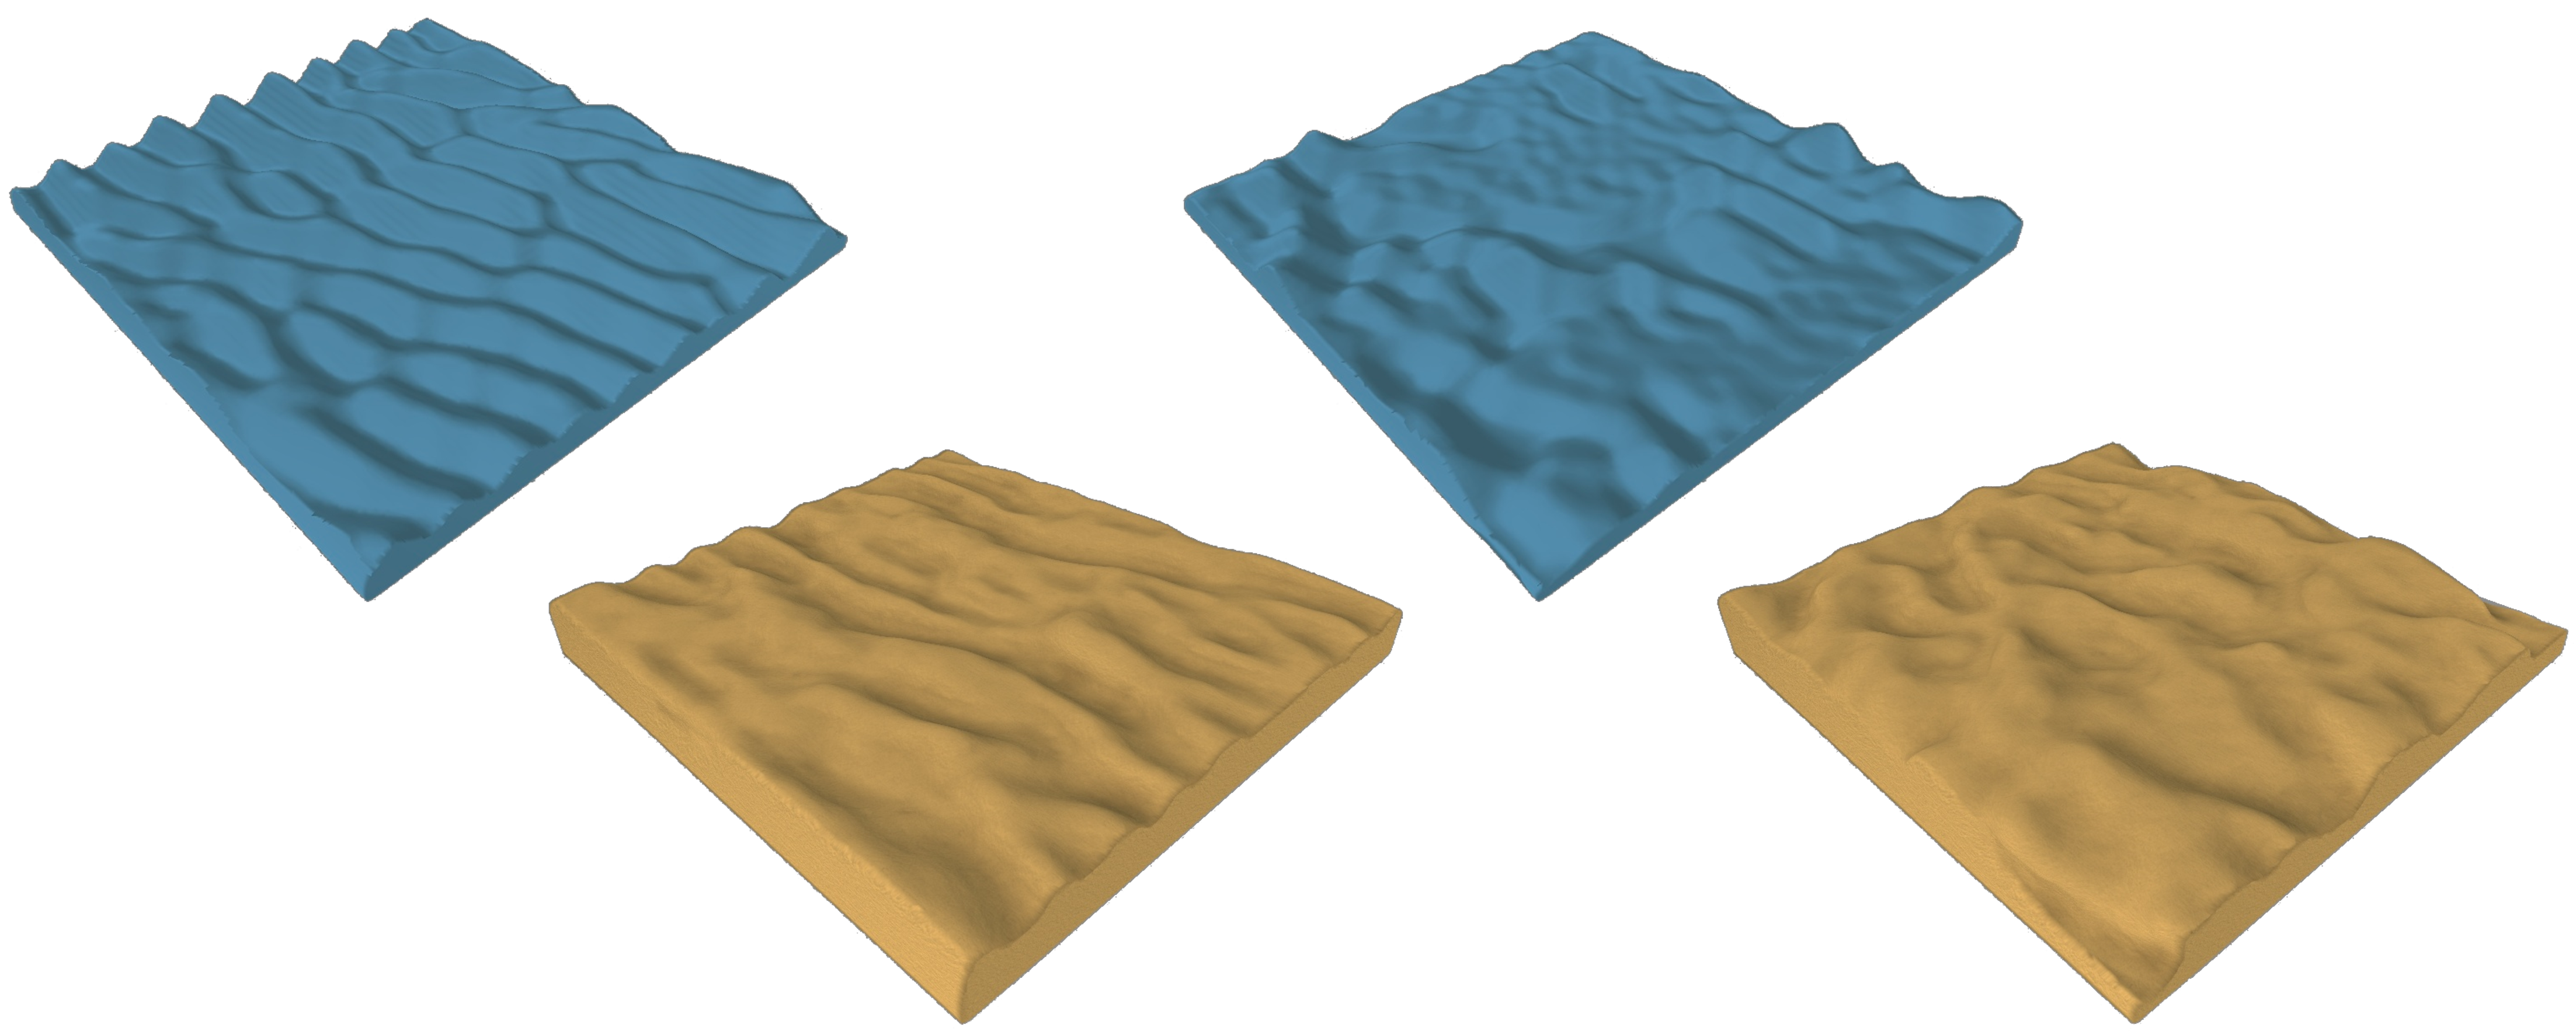
\includegraphics[width=\linewidth]{otherPapersRepro/desert.pdf}
\caption{The algorithm from Paris 2020 allow the generation of desertscapes (top), which we can (at least partially) reproduce with our erosion simulation (bottom). The different effects are achieved by affecting the wind direction and strength. }
\label{fig:screen-paris2020}
\end{figure}

\section{Discussion}
This work is a generalization of erosion that is applicable to any terrain representation. In practice, while similar particle physics is used on different terrain representations, using similar parameters does not ensure resulting in the same eroded terrain. Surfaces and normals being approximated differently have rippling effect on particle trajectories. 
Note that, not all effects can be applied to all representations, forinstance, karsts generation on 2.5D data structures. 

\textit{Realism}
Realism of the erosion simulation is highly correlated to the size and quantity of particles used and their distribution. Using too few or distributing them too sparsely will result in a terrain that is unrealistic since the alteration will have localized effects, breaking process homogeneity. \\ 
The resolution is also limited by the number and size of the particles, which can be problematic on implicit terrains that can theoretically have a infinite resolution.\\
Our method allows to perform erosion on implicit terrains. However, in its current form, our algorithm is time expensive on implicit representations since a large number of primitives are added in the composition tree. Using skeletons-defined primitives \cite{Hong2013, Rigaudiere2000}%, Schroeder1994}
 from particles trajectories and erosion/deposition values could be a solution to optimize the computation time.

\textit{Usage of velocity fields}
In our erosion algorithm, we simplify particle physics to enhance computational efficiency and facilitate parameterization. We use the velocity field from fluid simulations to approximate particle velocities. Sediment mass is harnessed to compensate for this approximation, allowing compatibility with various fluid simulation algorithms. Velocity fields can be recomputed at a frequency meeting the applications needs, ranging from "classic erosion simulation" (recomputed at each time step) to "simple simulation" (never recomputed). We addressed provisional adjustments to mitigate discrepancies when terrain changes due to erosion are not reflected in a static velocity field in section “3.3 Transport”. However, it is important to note that these are expedient solutions and may not fully capture precise dynamics of an evolving terrain. 

\textit{Performances}
To facilitate parallelization, we intentionally overlook particle interactions and sediment exchanges, albeit at the expense of achieving smoother results. Surface collisions are simplified to basic bounces with a damping parameter instead of relying on complex particles and ground properties (Young’s modulus, friction, material, ...)\cite{Yan2020}, further easing the parameterization process. However, these simplifications, combined with the inherent discrete nature of particles, as opposed to the continuous nature of erosion, result in a correlation between realism and particle count. \\
The performance of our method is influenced by the time required for collision detection. Consequently, we mainly observe better performances with explicit terrain models than with implicit models. 

\textit{Particle's atomicity}
While we can replicate various effects, the "fan" shape commonly observed in natural erosion patterns is not perfectly represented. This limitation arises because we do not account for the splitting of a particle, a process that significantly influences the multidirectional dislocation and trajectory of individual particles \cite{Ranz1960}. Additionally, we acknowledge an issue where particles may collide with the ceiling and the deposition is stuck. While a potential resolution involves splitting particles upon impact rather than simply depositing sediments, this introduces complexities to the parallelization layer of the method. Allowing particles to split introduces unpredictability in the total number of particles that will exist in the simulation. This unpredictability can complicate the use of multi-threading. Future works includes finding a data structure allowing this splitting efficiently, leading to more realistic erosion patterns.

\textit{Simulation with multiple materials}
One aspect we haven't addressed is a layered terrain with multiple materials. In the native way our method is done, we do not consider the transport of different materials (all sediments are considered as sand), but by storing a list of the different materials and the quantity transported by each particle, the same simulation process could be done at the cost of some memory and performance overhead. \\
Another possible adaptation of the erosion strategy for material voxels is to extend the erosion computation from binary voxels by define transformation rules from one material to another when a voxel is eroded a number $\#hits < -C$ or $\#hits > C$. For example, the material "clay" may transform to "sand" when eroded or to "rock" when many depositions occurred. 
\section{Conclusion}
\label{sec:conclusion}
We introduced a flexible particle-based erosion system that is easy to use and simple to implement. We have presented how to adapt the process for various terrain representations and generate a variety of erosion phenomenon due to rain, wind, water bodies... by adjusting intuitive parameters hence generate automatically realistic 2.5D and 3D terrains. The use of external velocity fields provides a high flexibility i.e. using the simulations that best fits the user's needs (precision, control, implementation efficiency...). 
Our method can also be applied to underwater environments with identical physics simulation since our erosion method can be applied on 3D representations. 
Erosion algorithms are often limited to the use of height fields, but by finding more generalized methods, we can go toward a global use of 3D terrains, which can offer richer and more diverse landscapes.

%
\section{Computation of a metaball}
\label{sec:appendix_metaball}
We use the following formula to evaluate a metaball in space with a center $c$ and of radius $R$:
$$ g(p) = 1 - \frac{||p - c||}{R} $$
using the euclidean distance.

We have a total amount $\totalErosion$ to define in this space, so the final metaball function $f$ needs to satisfy the equations \eqref{eq:function_f_is_metaball} and \eqref{eq:int_function_f_is_erosion}:
\begin{align}
\label{eq:function_f_is_metaball}
f(p) &= \lambda g(p) \\
\label{eq:int_function_f_is_erosion}
\int_{p \in V_{3D}}{f \, dp} &= \totalErosion
\end{align}

First, let's exploit the radial symmetry of the metaball and rewrite $g(p) = 1 - r$ by using the polar coordinates of the point $p - c$.

We can then integrate $g$ over the volume $V_{3D}$ as 
\begin{align}
&\int_{0}^{1}{ \int_{0}^{\pi}{ \int_{0}^{2\pi}{ g(r) r^2 \sin(\theta)\, dr} \, d\theta} \, d\phi} \nonumber \\
= &\int_{0}^{1}{ \int_{0}^{\pi}{ \int_{0}^{2\pi}{ (1 - r) r^2 \sin(\theta)\, dr} \, d\theta} \, d\phi} \nonumber \\
&= \int_{0}^{1}{ (1 - r)r^2 \, dr} \times \int_{0}^{\pi}{ \sin{\theta} \, d\theta } \times \int_{0}^{2\pi}{ 1 \, d\phi} \nonumber
\end{align}

We then break down the integrals one by one such as 
$$ \int_{0}^{1}{ (1 - r)r^2 \, dr} = \frac{1}{12} \nonumber$$ 
$$ \int_{0}^{\pi}{ \sin{\theta} \, d\theta } = 2 \nonumber$$ 
$$ \int_{0}^{2\pi}{ 1 \, d\phi} = 2 \pi \nonumber$$

By combining all these integrals, we get $\int{g} = \frac{1}{12} \times 2 \times 2\pi = \frac{\pi}{3}$.

So given $\int{f} = \erosionAmount$ and $\int{f} = \lambda \int{g}$, we can deduce that $\lambda = \frac{\totalErosion}{\int{g}} = \frac{3}{\pi}\totalErosion$.

From \eqref{eq:function_f_is_metaball} we finally get 
\begin{align} 
\label{eq:proofErosionMetaball}
f(p) = \frac{3 \totalErosion}{\pi} \left(1 - \frac{||p - c||}{R} \right)
\end{align}
, representing the rate of change on the evaluation function of the terrain surface.

The integration in the voxel space is out of the scope of this paper and a numerical solution is instead proposed in Section~\ref{sec:application_on_voxels}.


    \clearpage
\begin{figure*}
	\includegraphics[width=\linewidth]{Results/results.pdf}
	\centering
	\caption{Erosion processes results on various representations presented in section \ref{sec:erosion_examples}. Used parameters used are detailed in  Table~\ref{tab:result_parameters}.}
	\label{tab:result_figures}
	
\end{figure*}
